%%% Load required packages here (note that many are included already).

% \usepackage{balance} % for balancing columns on the final page
% \usepackage{amsmath,amsfonts}
% \usepackage{algorithmic}
% \usepackage{algorithm}
% \usepackage{array}
% \usepackage[caption=false,font=normalsize,labelfont=sf,textfont=sf]{subfig}
% \usepackage{textcomp}
% \usepackage{stfloats}
% \usepackage{url}
% \usepackage{verbatim}
% \usepackage{graphicx}
% \usepackage{cite}
% \usepackage[mode=buildnew]{standalone}
% \usepackage{tikz}
% \usepackage{kbordermatrix}
% \usetikzlibrary{positioning, shapes, arrows, tikzmark,decorations.pathreplacing}
% \tikzstyle{curly} = [decorate,decoration={brace,amplitude=10pt}]
% \usepackage{mathrsfs}


% % Definitions of handy macros can go here
% \newcommand{\swap}[3][-]{#3#1#2} % just an example
% %\usepackage{amssymb}
% \input{macros}
% %\usepackage{caption}
% \usepackage{amsmath,array}
% \newcommand{\dataset}{{\cal D}}
% \newcommand{\fracpartial}[2]{\frac{\partial #1}{\partial  #2}}
% \usepackage{mathtools}
% %\usepackage{amssymb}
% \usepackage{bm}
% \usepackage[mode=buildnew]{standalone}
% \usepackage{hyperref}
% \usepackage{natbib}
% \newtheorem{theorem}{Theorem}[section]
% \newtheorem{corollary}{Corollary}[theorem]
% \newtheorem{lemma}[theorem]{Lemma}
% \newtheorem{assumption}{Assumption}
% \newtheorem{example}{Example}
% \newtheorem{remark}{Remark}
%\newenvironment{proof}{\paragraph{Proof:}}{\hfill$\square$}


% command for comment boxes

% \definecolor{wheat}{rgb}{0.96,0.87,0.70}
% \definecolor{lightblue}{rgb}{0.8,0.8,1}
% \definecolor{lightred}{rgb}{1,0.8,0.8}
% \definecolor{lightgreen}{rgb}{0.8,1,0.8}
% \newcommand{\todo}[1]{
% 	\begin{center}
% 		\fcolorbox{wheat}{wheat}{\parbox[t]{0.9\linewidth}{\textbf{ToDo:} #1}}
% \end{center}}
% \newcommand{\tommy}[1]{
% 	\begin{center}
% 		\fcolorbox{lightblue}{lightblue}{\parbox[t]{0.9\linewidth}{\textbf{Tommy:} #1}}
% \end{center}}
% \newcommand{\hannes}[1]{
% 	\begin{center}
% 		\fcolorbox{lightred}{lightred}{\parbox[t]{0.9\linewidth}{\textbf{Hannes:} #1}}
% \end{center}}
% \newcommand{\deba}[1]{
% 	\begin{center}
% 		\fcolorbox{lightgreen}{lightgreen}{\parbox[t]{0.9\linewidth}{\textbf{Deba:} #1}}
% \end{center}}

%%%%%%%%%%%%%%%%%%%%%%%%%%%%%%%%%%%%%%%%%%%%%%%%%%%%%%%%%%%%%%%%%%%%%%%%

%%% AAMAS-2023 copyright block (do not change!)

\newcommand {\matr}[2]{\left[\begin{array}{#1}#2\end{array}\right]}
\newcommand{\E}{\mathbb{E}}
\newcommand{\tr}{\mathrm{tr}}
\newcommand{\x}{{\mathbf{x}}}
\renewcommand{\u}{{\mathbf{u}}}
\newcommand{\w}{{\mathbf{w}}}
\renewcommand{\r}{{\mathbf{r}}}

\definecolor{wheat}{rgb}{0.96,0.87,0.70}
\definecolor{lightblue}{rgb}{0.8,0.8,1}
\definecolor{lightred}{rgb}{1,0.8,0.8}
\definecolor{lightgreen}{rgb}{0.8,1,0.8}

% \newcommand\argmax{\mathop{\rm arg\,max}}
% \newcommand\argmin{\mathop{\rm arg\,min}}
% \newcommand {\defn} {\triangleq}
% \newcommand \Reals {\ensuremath{\mathbb{R}}}
% \newcommand \E {\mathop{\mbox{\ensuremath{\mathbb{E}}}}\nolimits}
% \newcommand \V {\mathop{\mbox{\ensuremath{\mathbb{V}}}}\nolimits}
% \renewcommand \Pr {\mathop{\mbox{\ensuremath{\mathbb{P}}}}\nolimits}
% %\newtheorem{lemma}{Lemma}
% %% macros for symbols
\newcommand \pol {\pi}
\newcommand \Pol {\Pi}
% \newcommand \bel {\beta}
\newcommand \mdp {\mu}
\newcommand \MDP {\mathcal{M}}
\newcommand \return {R}
\newcommand \utility {U}
\newcommand \GP {\mathcal{GP}}
\newcommand \param {\theta} %% unknown parameter
\newcommand \Params {\Theta} %% unknown parameter



\newcommand \disc {\gamma}
\newcommand \MDPs {\mathcal{M}} %% The MDP
\newcommand \Pols {\Pi} %% The policy
\newcommand \VC[3] {V_{#1,#2}^{#3}}
\newcommand \VS[2] {V_{#1,#2}^{*}}
\newcommand \CS {\mathcal{S}} %% The state space
\newcommand \CA {\mathcal{A}} %% The action space
\newcommand \CV {\mathcal{V}} %% The value function estimate
\newcommand \trans {\mathcal{T}} %% The transition kernel
\newcommand \rew {\rho} %% The reward function\newcommand \disc {\gamma} %% discount factor
\newcommand \abel {\hat{\xi}} %% approximate belief
\newcommand \mbel {\psi} %% belief about MDPs 

\newcommand \p {\partial}

\newcommand \Bellman {\mathscr{L}}
\newcommand \PBellman {\mathscr{P}}
\newcommand \util {U}
\newcommand \val {\vectorsym{v}}
\newcommand \Vals {\mathcal{V}}
\newcommand \discount {\gamma}
\newcommand \horizon {T}

%% Commands

% \DeclareMathOperator{\st}{s.t.\,}
% \DeclareMathOperator{\trace}{tr}

\newcommand \onenorm[1]{\left\|#1\right\|_1}
\newcommand \pnorm[2]{\left\|#1\right\|_{#2}}
\newcommand \inftynorm[1]{\left\right\|#1\|_\infty}
\newcommand \norm[1]{\left\|#1\right\|}


\newcommand \dd {\, \mathrm{d}}
\let\Pr\relax
\newcommand \Pr {\mathbb{P}}

\newcommand \cset[2] {\left\{#1 ~\middle|~ #2\right\}}
\newcommand \set[1] {\left\{#1\right\}}
\newcommand \ind[1] {\mathds{1}\left\{#1\right\}}

\newcommand \KL[2] {D\left( #1 ~\middle\|~ #2\right)}

% \DeclareMathAlphabet{\mathpzc}{OT1}{pzc}{m}{it}

\newcommand \Softmax {{\mathpzc{Softmax}}}
\newcommand \GammaDist {{\mathpzc{Gamma}}}
\newcommand \Dirichlet {{\mathpzc{Dir}}}
\newcommand \Uniform {{\mathpzc{Unif}}}
\newcommand \Bernoulli {{\mathpzc{Bern}}}
\newcommand \Binomial {{\mathpzc{Binom}}}
\newcommand \Beta {{\mathpzc{Beta}}}
\newcommand \Geometric {{\mathpzc{Geom}}}
\newcommand \Normal {{\mathpzc{N}}}
\newcommand \Multinomial {{\mathpzc{Mult}}}
\newcommand \Wishart {{\mathpzc{Wish}}}


\if 1
\newcommand \note[2][blue] {{\color{#1} \texttt{[#2]}}}
\newcommand \cor[2][red] {{\color{#1}#2}}
\newcommand \ins[2][magenta] {{\color{#1}#2}}
\newcommand \del[2][red] {{\color{#1}\sout{#2}}}
\newcommand \grm[2][green!50!black] {{\color{#1}#2}}
\else

\newcommand \ins[2][magenta] {{\color{#1}#2}}
\fi

%%% Use this environment to specify a short abstract for your paper.

\begin{abstract}
	For deploying model-based reinforcement learning in the wild, we aim to compute an efficient policy for an unseen Markov Decision Process (MDP) setting, where we do not have access to an explicit model. But due to availability of either simulators or data for similar tasks, we often can build accurate MDP models for similar problem settings (or tasks), which might differ slightly from the target MDP. 
	In this paper, we study the problem of transferring the available MDP models to learn and plan efficiently in an unknown but similar MDP. We refer to it as \textit{Model Transfer Reinforcement Learning (MTRL)} problem. 
	
	First, we formulate MTRL for discrete MDPs and Linear Quadratic Regulators (LQRs) with continuous state-actions.
	Then, we propose a generic two-stage algorithm, MLEMTRL, to address the MTRL problem in both the discrete and continuous settings. In the first-stage, MLEMTRL uses a \textit{constrained Maximum Likelihood Estimation (MLE)}-based approach to estimate the target MDP model using a set of known MDP models. In the second-stage, using the estimated target MDP model, MLEMTRL deploys a model-based planning algorithm appropriate for the MDP class.
	Theoretically, we prove worst-case regret bounds for MLEMTRL both in realisable and non-realisable settings.
	We empirically demonstrate that MLEMTRL allows faster learning in new MDPs than learning from scratch and also achieves near-optimal performance depending on the similarity of the available MDP models and the target MDP.
\end{abstract}


% \keywords{Reinforcement Learning, Transfer Learning, Maximum Likelihood Estimation, Linear Quadratic Regulator}


% \newcommand{\BibTeX}{\rm B\kern-.05em{\sc i\kern-.025em b}\kern-.08em\TeX}



\section{Introduction}\label{sec:intro}

%%% GENERAL OVERVIEW
Deploying autonomous agents in the real world poses a wide variety of challenges. As in~\citep{dulac2021challenges}, we are often required to learn the real-world model with limited data, and use it to plan to achieve satisfactory performance in the real world. There might also be safety and reproducibility constraints, which require us to track a model of the real-world environment~\citep{skirzynski2021automatic}.
In light of these challenges, we attempt to construct a framework that can aptly deal with optimal decision making for a novel task, by leveraging external knowledge. As the novel task is unknown, we adopt the Reinforcement Learning (RL)~\citep{sutton2018reinforcement} framework to guide an agent's learning process and to achieve near-optimal decisions.
%of decision-making under uncertainty, %which has a deep history going back to~\citep{von2007theory}, to operations research~\citep{bell1982regret} to learning~\citep{bertsekas1997nonlinear}. One such approach that we adopt in this work, is the Reinforcement Learning (RL)~\citep{sutton2018reinforcement} framework to guide an agent's learning process and to achieve near1-optimal decisions. 

An RL agent interacts directly with the environment to improve its performance. Specifically, in model-based RL, the agent tries to learn a model of the environment and then use it to improve performance~\citep{moerland2020model}. In many applications, the depreciation in performance due to sub-optimal model learning can be paramount. For example, if the agent interacts with living things or expensive equipment, decision-making with an imprecise model might incur significant cost~\citep{polydoros2017survey}. In such instances, boosting the model learning by leveraging external knowledge from the existing models, such as simulators~\citep{peng2018sim}, physics-driven engines, etc., can be of great value~\citep{taylor2008transferring}. A model trained on simulated data may perform reasonably well when deployed in a new environment, given the novel environment is \emph{similar enough} to the simulated model. 
Also, RL algorithms running on different environments yield data and models that can be used to plan in another similar enough real-life environment.
In this work, we study the problem where we have access to multiple source models built using simulators or data from other environments, and we want to transfer the source models to perform efficient model-based RL in a different real-life environment.

% \begin{example}
Let us consider that a company is designing autonomous driving agents for different countries in the world. The company has designed two RL agents that have learned to drive well in USA and UK. Now, the company wants to deploy a new RL agent in India. Though all the RL agents are concerned with the same task, i.e. driving, the models encompassing driver behaviors, traffic rules, signs, etc., can differ for each. For example, UK and India have left-handed traffic, while the USA has right-handed traffic.  However, learning a new controller \emph{specifically} for every new geographic location is computationally expensive and time-consuming, as both data collection and learning take time. Thus, the company might use the models learned for UK and USA, to estimate the model for India, and use it further to build a new autonomous driving agent (RL agent). Hence, being able to transfer the source models to the target environment allows the company to use existing knowledge to build an efficient agent faster and resource efficiently.
%Consider the case where an autonomous driving agent has learned how to drive in the US but now is tasked with driving in the UK. Should you expect it to perform well in both cases? Disregarding the fact of right-hand vs. left-hand traffic, the traffic rules, signs and driver behavior may differ. However, learning a new controller \emph{specifically} for every new geographic location is intractable. Being able to use existing knowledge obtained from one agent to bootstrap learning of a new agent may very well be a good compromise in this setting.\dbcomment{edit it with one more source model}
% \end{example}

%%% CONTRIBUTION
\textit{We address this problem of model transfer from source models to a target environment to plan efficiently.} We observe that this problem falls at the juncture of \emph{transfer learning} and \emph{reinforcement learning}~\citep{taylor2009transfer,lazaric2012transfer,laroche2017transfer}. %allows us to bootstrap learning of new agents in novel environments. 
%Our work is positioned within the field of TRL, which has been investigated thoroughly. 
\citep{lazaric2012transfer} enlists three approaches to transfer knowledge from the \emph{source tasks} to a \emph{target task}. (i) \emph{Instance transfer:} data from the source tasks is used to guide decision-making in the novel task~\citep{taylor2008transferring}. (ii) \emph{Representation transfer:} a representation of the task, such as learned neural network features, are transferred to perform the new task~\citep{zhang2018decoupling}. (iii) \emph{Parameter transfer:} the parameters of the RL algorithm or \emph{policy} are transferred~\citep{rusu2015policy}. In our paper, the source tasks are equivalent to the source models, and the target task is the target environment. Moreover, we adopt the \textbf{model transfer reinforcement learning} approach (MTRL), which encompasses both (i) and (ii) (Section~\ref{sec:trl}). 

\citep{langley2006transfer} describes three possible benefits of transfer learning. The first is~\textbf{learning speed improvement}, i.e. decreasing the amount of data required to learn the solution. Secondly, \textbf{asymptotic improvement}, where the solution results in better asymptotic performance. Lastly, \textbf{jumpstart improvement}, where the initial proxy model serves as a better starting solution than that of one learning the true model from scratch. In this work, we propose a new algorithm to transfer RL that achieves both learning speed improvement and jumpstart improvement (Section~\ref{sec:experiments}). However, we might not find an asymptotic improvement in performance if compared with the best and unbiased algorithm in the true setting. Rather, we aim to achieve a model estimate that allows us to plan accurately in the target MDP (Section~\ref{sec:bounds}).%\\ %Indeed, from our problem formulation the reason for this will be clear and for many settings not only will we attain near-optimal performance but actual optimal performance.

\noindent\textbf{Contributions.} We aim to answer two central questions:
\begin{enumerate}
    \item  \emph{How can we accurately construct a model using a set of source models for an RL agent deployed in the wild?} 
    \item \emph{Does the constructed model allow efficient planning and yield improvements over learning from scratch?}
\end{enumerate}
In this paper, we address these questions as follows:\\
\noindent1. \textit{A Taxonomy of MTRL:} First, we formulate the problem with the Markov Decision Processes (MDPs). % setting of RL. 
We further provide a taxonomy of the problem depending on a discrete or continuous set of source models, and whether the target model is realisable by the source models (Section~\ref{sec:trl}).%\\

\noindent2. \textit{Algorithm Design with MLE:} Following that, we design a two-stage algorithm MLEMTRL to plan in an unknown target MDP (Section~\ref{sec:algorithms}). In the first stage, MLEMTRL uses a Maximum Likelihood Estimation (MLE) approach to estimate the target MDP using the source MDPs. In the second stage, MLEMTRL uses the estimated model to perform model-based planning. We instantiate MLEMTRL for discrete state-action (tabular) MDPs and Linear Quadratic Regulators (LQRs). We also derive a generic bound on the goodness of the policy computed using MLEMTRL (Section~\ref{sec:bounds}). We further provide a meta-algorithm, called Meta-MLEMTRL, to control the adaptation to the non-realisable setting (Section~\ref{sec:meta_mlemtrl}).%\\

\noindent3. \textit{Performance Analysis:} In Section~\ref{sec:experiments}, we empirically verify whether MLEMTRL improves the performance for unknown tabular MDPs and LQRs than learning from scratch. MLEMTRL exhibits learning speed improvement for tabular MDPs and LQRs. For LQRs, it incurs learning speed improvement and asymptotic improvement. We also observe that the more similar the target and source models are, the better the performance of MLEMTRL, as indicated by the theoretical analysis. An ablation study of Meta-MLEMTRL under realisable and non-realisable settings further shows provable improvements yielded in the asymptotic and non-realisable regimes.%\\ %improvements obtained using MLEMTRL depend on the similarity between the target and source models. 

% This is accomplished through the transfer reinforcement learning framework, by efficiently making use of knowledge from source tasks when interacting with the target task. The proposed algorithm, MLEMTRL, displays superiority compared to an agent learning the novel task from scratch for two of the main objectives listed by~\citep{taylor2009transfer}, namely, jumpstart improvement and learning speed improvement. We demonstrate the performance of the algorithm in a tabular and LQR setting and prove worst-case regret bounds for the algorithm in both the realisable and non-realisable settings. Finally, we show a connection between model dissimilarity and degradation in performance, indicating transfer reinforcement learning makes the most sense when the tasks are similar.

% \textbf{Outline.}
% In this work, we begin by introducing the necessary background knowledge of MDPs and the appropriate likelihood functions for said MDP classes, in Section~\ref{sec:background}. Next, we instantiate the \emph{transfer reinforcement learning} problem in Section~\ref{sec:trl} and the various sub-settings of the problem. Further, we describe how to achieve optimality (or near-optimality) in this setting. Later, in Section~\ref{sec:algorithms}, we introduce the proposed algorithm, MLEMTRL, and the two-stage process it contains. Namely, \emph{model identification} and \emph{model-based planning}. In Section~\ref{sec:bounds} we provide theoretical worst-case bounds for the proposed algorithm and empirical results in Section~\ref{sec:experiments}. Finally, in Section~\ref{ch:discussion} we summarise our findings and describe future directions of this work.

Before elaborating on the contributions, we posit this work in the existing literature (Section~\ref{sec:related}) and discuss the background knowledge of MDPs and MLEs (Section~\ref{sec:background}).

\section{Related Work}\label{sec:related}
Our work on Model Transfer Reinforcement Learning is situated in the field of Transfer RL (TRL) and also is closely related to the multi-task RL and Bayesian multi-task RL literature. In this section, we elaborate on these connections.

TRL is widely studied in Deep Reinforcement Learning. \citep{zhu2023transfer} introduces different ways of transferring knowledge, such as \emph{policy transfer}, where the set of source MDPs $\mathcal{M}_s$ has a set of expert policies associated with them. The expert policies are used together with a new policy for the novel task by transferring knowledge from each policy. \citep{rusu2015policy} uses this approach, where a student learner is combined with a set of teacher networks to guide learning in multi-task RL. \citep{parisotto2015actor} develops an actor-critic structure to learn ways to transfer its knowledge to new domains.   \citep{arnekvist2019vpe} invokes generalisation across Q-functions by learning a master policy. Here,\textit{ we focus on model transfer instead of policy}.

Another seminal work in TRL, by~\citep{taylor2009transfer} distinguishes between \emph{multi-task learning} and \emph{transfer learning}. Multi-task learning deals with problems where the agent aims to learn from a distribution over scenarios, whereas transfer learning makes no specific assumptions about the source and target tasks. Thus, in transfer learning, the tasks could involve different state and action spaces and different transition dynamics. Specifically, we focus on \textbf{model-transfer}~\citep{atkeson1997comparison} approach to TRL, where the state-action spaces and also dynamics can be different. \citep{atkeson1997comparison} performs model transfer for a target task with an identical transition model. Thus, the main consideration is to transfer knowledge to tasks with the same dynamics but varying rewards. \citep{laroche2017transfer} assumes a context similar to that of~\citep{atkeson1997comparison}, where the model dynamics are identical across environments. In our work, we rather assume that the reward function is the same, but the transition models are different. We believe this is an interesting question as the harder part of learning an MDP is learning the transition model. 
These works explicate a deep connection between the fields of \emph{multi-task learning} and \emph{TRL}. In general, TRL can be viewed as an extension of multi-task RL, where multiple tasks can either be learned simultaneously or have been learned \textit{a priori}. This flexibility allows us to learn even in settings where the state-actions and transition dynamics are different among tasks. \citep{rommel2017aircraft} describes a multi-task Maximum Likelihood Estimation procedure for optimal control of an aircraft. They identify a mixture of Gaussians, where the mixture is over each of the tasks. Here, we adopt an MLE approach to TRL to optimise performance for the target MDP (or a target task) rather than restricting to a mixture of Gaussians.

The Bayesian approach to multi-task RL~\citep{wilson2007multi, lazaric2010bayesian} tackles the problem of learning jointly how to act in multiple environments. \citep{lazaric2010bayesian} handles the \emph{open-world assumption}, i.e. the number of tasks is unknown. This allows them to transfer knowledge from existing tasks to a novel task, using value function transfer. However, this is significantly different from our setting, as we are considering model-based transfer. Further, \textit{we adopt an MLE-based framework in lieu of the full Bayesian procedure described in their work}.
In Bayesian RL, \citep{tamar2022regularization} also investigates a learning technique to generalise over multiple problem instances. By sampling a large number of instances, the method is expected to learn how to generalise from the existing tasks to a novel task. We do not assume access to such prior or posterior distributions to sample from.

There is another related line of work, namely multi-agent transfer RL~\citep{da2019survey}. For example, \citep{liang2023federated} develops a TRL framework for autonomous driving using federated learning. They accomplish this by aggregating knowledge for independent agents. This setting is different from general transfer learning but could be incorporated if the source tasks are learned simultaneously with the target task. This requires cooperation among agents, which is out of the scope.% of the paper.

%\newpage
\section{Background}\label{sec:background}

In this section, we introduce the important concepts on which this work is based upon. Firstly, we introduce the way we model the dynamics of the tasks. Secondly, we describe the Maximum Likelihood Estimation (MLE) framework used in this work.

\subsection{Markov Decision Process}\label{sec:mdp}
We study sequential decision-making problems that can be represented as Markov Decision Processes (MDPs)~\citep{puterman2014markov}. An MDP $\mdp$ consists of a discrete or continuous state space denoted by $\mathcal{S}$, a discrete or continuous action-space $\mathcal{A}$, a reward function $\mathcal{R} : \mathcal{S} \times \mathcal{A} \rightarrow \mathbb{R}$ which determines the quality of taking action $a$ in state $s$, and a transition function $\mathcal{T} : \mathcal{S} \times \mathcal{A} \rightarrow \Delta\mathcal{S}$ inducing a probability distribution over the successor states $s'$ given a current state $s$ and action $a$. Finally, in the infinite-horizon formulation, a discount factor $\gamma \in [0, 1)$ is assigned. The overarching objective for the agent is to compute a decision-making policy $\pol : \mathcal{S} \rightarrow \Delta(\mathcal{A})$ that maximises the expected sum of future discounted rewards up until the horizon $T$: $V_\mdp^{\pol}(s) = \mathbb{E}\Big[\sum_{t=0}^T \gamma^t \mathcal{R}(s_t, a_t)\Big]$. $V_\mdp^{\pol}(s)$ is called the value function of policy $\pol$ for MDP $\mdp$. The optimal value function is denoted as $\mdp$ is $V_\mdp^{*} = V_\mdp^{\pol^{*}}$. The technique used to obtain the the optimal policy $\pol^{*} = \underset{\pol}{\sup} \, V_\mdp^{\pol}$ depends on the MDP class. The MDPs with discrete state-action spaces are referred to as tabular MDPs. In this paper, we also study a specific class of MDPs with continuous state-action spaces, namely the Linear Quadratic Regulators (LQRs)~\citep{kalman1960new}. In tabular MDPs, we employ \textsc{ValueIteration}~\citep{puterman2014markov} for model-based planning whereas in the LQR setting we use \textsc{RiccatiIteration}~\citep{willems1971least}. 

The standard metric used to measure the performance of a policy $\pol$~\citep{bell1982regret} for an MDP $\mdp$ is \textit{regret} $R(\mdp, \pol)$. Regret is the difference between the optimal value function and the value function of $\pol$. In this work, we extend the definition of regret for MTRL, where the optimality is taken with respect to a policy class in the target MDP.


\subsection{Maximum Likelihood Estimation}
One of the most popular methods of constructing point estimators is the \emph{Maximum Likelihood Estimation} (MLE)~\citep{casella2021statistical} framework. Given a density function $f(x \, | \, \theta_1, \hdots, \theta_n)$ and associated i.i.d. data $X_1, \hdots, X_t$, the goal of the MLE scheme is to maximise,
\begin{equation}\label{eq:mle}
\hspace*{-1em}  \ell(\theta \, | \, x) \triangleq \ell(\theta_1, \hdots, \theta_n \, | \, x_1, \hdots, x_t) \triangleq \log \prod_{i=1}^t f(x_i \, | \, \theta_1, \hdots, \theta_n).
\end{equation}
$\ell(\cdot)$ is called the log-likelihood function. The set of parameters maximising Equation~\ref{eq:mle} is called the \emph{maximum likelihood estimator} of $\theta$ given the data $X_1, \hdots, X_t$. Maximum likelihood estimation has many desirable properties that we leverage in this work. For example, the ML estimator satisfies \emph{consistency}, i.e. under certain conditions, it achieves optimality even for \emph{constrained} MLE. An estimator being consistent means that if the data $X_1, \hdots, X_t$ is generated by $f(\cdot \, | \, \theta)$ and as $t\rightarrow \infty$, the estimate almost surely converges to the true parameter $\theta$. \citep{kiefer1956consistency} shows that MLE admits the consistency property given the following assumptions hold. The model is \emph{identifiable}, i.e. the densities at two parameter values must be different unless the two parameter values are identical. Further, the parameter space is \emph{compact} and \emph{continuous}. Finally, if the log-density is \emph{dominated}, one can establish that MLE converges to the true parameter almost surely~\citep{newey1987asymmetric}.
For problems where the likelihood is unbounded, flat or otherwise unstable one may introduce a penalty term in the objective function. This approach is called \emph{penalised maximum likelihood estimation}~\citep{ciuperca2003penalized, ouhamma2023bilinear}. As we in our work are mixing over known parameters, we do not need to add regularisation to our objective to guarantee convergence.

In this work, we iteratively collect data and compute new point estimates of the parameters and use them in our decision-making procedure. In order to carry out MLE, a likelihood function has to be chosen. In this work, we investigate two such likelihood functions in Section~\ref{sec:algorithms}, one for each respective model class. 
%\vspace*{-1em}\section{A Taxonomy of Model Transfer RL}\label{sec:trl}
\section{A Taxonomy of Model Transfer RL}\label{sec:trl}
Now, we formally define the Model Transfer RL problem and derive a taxonomy of settings encountered in MTRL.

\subsection{MTRL: Problem Formulation}
Let us assume that we have access to a set of source MDPs $\mathcal{M}_s \triangleq \{\mu_i\}_{i=1}^m$. The individual MDPs can belong to a finite or infinite but compact set depending on the setting. For example, for tabular MDPs with finite state-actions, this is always a finite set. Whereas for MDPs with continuous state-actions, the transitions can be parameterised by real-valued vectors/matrices, corresponding to an infinite but compact set.
Given access to $\mathcal{M}_s$, we want to find an optimal policy for an unknown target MDP $\mdp^*$ that we encounter while deploying RL in the wild.
At each step $t$, we use $\mathcal{M}_s$ and the data observed from the target MDP $D_{t-1} \triangleq \{ s_0, a_0, s_1, \ldots, s_{t-1}, a_{t-1}, s_t\}$ to construct an estimate of $\mdp^*$, say $\hat{\mdp}^t$. Now, we use $\hat{\mdp}^t$ to run a model-based planner, such as \textsc{ValueIteration} or \textsc{RiccatiIteration}, that leads to a policy $\pol^t$. After completing this planning step, we interact with the target MDP using $\pol_t$ that yields an action $a_t$, and leads to observing $s_{t+1}, r_{t+1}$. We update the dataset with these observations: $D_t \triangleq D_{t-1} \cup \{a_{t}, s_t\}$. Here, we assume that all the source and target MDPs share the same reward function $\mathcal{R}$. We do not restrict the state-action space of target and source MDPs. %$\mathcal{S}_{\mathrm{target}} \times \mathcal{A}_{\mathrm{target}}$

Our goal is to compute a policy ${\pol}^t$ that performs as close as possible with respect to the optimal policy $\pol^*$ for the target MDP as the number of interactions with the target MDP $t\rightarrow \infty$.
This allows us to define a notion of regret for MTRL: $R(\mdp^{*}, \pol_t) \triangleq V_{\mdp^{*}}^{*}-V_{\mdp^{*}}^{\pol_t}$. Here, $\pol_t$ is a function of the source models $\mathcal{M}_s$, the data collected from target MDP $D_t$, and the underlying MTRL algorithm.
The goal of an MTRL algorithm is to minimise $R(\mdp^{*}, \pol_t)$.
For the parametric policies $\pol_{\theta}$ with $\theta \in \Theta \subset \mathbb{R}^d$, we can specialise the regret further for this parametric family: $R(\mdp^{*}, \pol_{\theta_t}) = V_{\mdp^{*}}^{\pol{\theta^*}}-V_{\mdp^{*}}^{\pol_{\theta_t}}$. For example, for LQRs, we by default work with linear policies. We use this notion of regret in our theoretical and experimental analysis.

%\cdcomment{Big picture: You do not define the model transfer problem at all. What is the criterion for a good transfer? Performance should depend on (a) the source MDPs (b) the target MDP (c) the number of episodes / horizon in the target MDP. Are you then comparing against the oracle policy of the target MDP? The mechanics of the transfer only seem to relate to (a) and (b)}

%\vspace*{-1em}\subsection{Three Classes of MTRL Problems}\vspace*{-.5em}
\subsection{Three Classes of MTRL Problems}
We begin by illustrating MTRL using Figure~\ref{fig:trl}. In the figure, the source MDPs $\mathcal{M}_s$ are depicted in red. This green area is the convex hull spanned by the source models $\mathcal{C}(\mathcal{M}_s)$. The target MDP $\mdp^{*}$, the best representative within the convex hull of the source models $\mdp$, and the estimated MDP $\hat{\mdp}$ are shown in blue, yellow, and purple, respectively. %The main takeaway of this figure is the location of the true model $\mdp^{*}$ relative to the source models. 
If the target model is \emph{inside} the convex hull, we call it a \textbf{realisable} setting. whereas If the target model is outside (as in Figure~\ref{fig:trl}), then we have a \textbf{non-realisable} setting.

Figure~\ref{fig:trl} also shows that the total deviation of the estimated model from the target model depends on two sources of errors: (i) realisability, i.e. how far is the target MDP $\mu^*$ from the convex hull of the source models $\mathcal{C}(\mathcal{M}_s)$ available to us, and (ii) estimation, i.e. how close is the estimated MDP $\hat{\mdp}$ to the best possible representation $\mdp$ of the target MDP. In the realisable case, the realisability gap can be reduced to zero, but not otherwise. This approach allows us to decouple the effect of the expressibility of the source models and the goodness of the estimator.
\setlength{\textfloatsep}{4pt}%
\begin{figure}
    \centering
    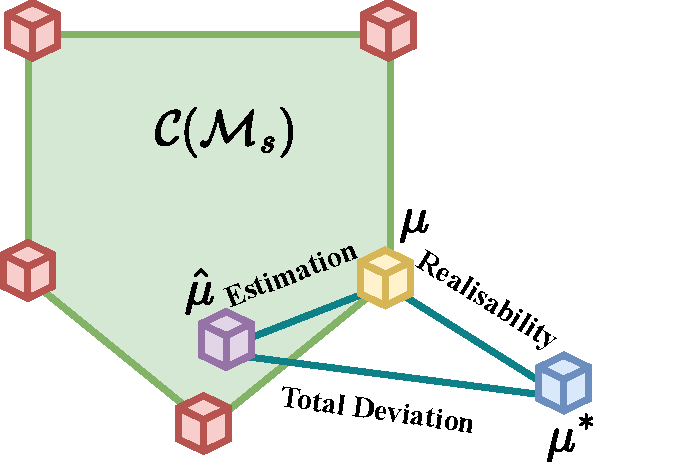
\includegraphics[width=0.35\paperwidth]{img/TRL.pdf}
    \caption{An illustration of the MTRL setting. The source models $\mathcal{M}_s$ are the red boxes. The green area is the convex hull $\mathcal{C}(\mathcal{M}_s)$ spanned by the source models. The target MDP $\mdp^{*}$ is displayed in blue, and the best proxy model is contained in the convex hull $\mdp$ in yellow. Finally, the estimator of the best proxy model $\hat{\mdp}$ is shown in purple.}
    \label{fig:trl}
\end{figure}
\iffalse
(a) \textbf{Finite and realisable setting:}  If the true model $\mdp^{*}$ is part of the convex hull spanned by the source models $\mdp^{*} \in \mathcal{C}(\mathcal{M}_s)$ and the optimisation over the possible models is taken directly over the source models, that is, the selected model $\hat{\mdp} \in \mathcal{M}_s$. Relating back to Figure~\ref{fig:trl}, optimisation is taken directly over the red boxes. 

(b) In the second setting, \textbf{infinite and realisable setting} the true MDP is again part of the convex hull $\mdp^{*} \in \mathcal{C}(\mathcal{M}_s)$. However, now the optimisation is taken over the convex hull. In Figure~\ref{fig:trl} this corresponds to the green area. 

(c) Thirdly, in the \textbf{infinite and non-realisable} setting, we have no guarantee the true MDP is part of the convex hull. In fact, it can be arbitrarily far away. Finally, we describe how we obtain (near)-optimality under the TRL framework and the measure of \emph{regret}.
\fi

%\subsection{MLE for The Three Classes of MTRL}
Now, we further elaborate on these three classes and the corresponding implications of performing MLE.

\textbf{I. Finite and Realisable Plausible Models.}\label{subsec:finite}
If the true model $\mdp^{*}$ is one of the target models, i.e. $\hat{\mdp} \in \mathcal{M}_s$, we have to identify the target MDP from a finite set of plausible MDPs. Thus, the corresponding MLE involves a finite set of parameters, i.e. the parameters of the source MDPs $\mathcal{M}_s$. We compute the MLE $\hat{\mdp}$ by solving the optimisation problem:
\begin{equation}
    \hat{\mdp} \in \underset{\mdp' \in \mathcal{M}_s}{\arg\max} \, \log \mathbb{P}(D_t \, | \, \mdp'), D_t \sim \mdp^{*}.
\end{equation}
This method may serve as a reasonable heuristic for the TRL problem, where the target MDP is the same as or reasonably close to one of the source MDPs. However, this method will potentially be sub-optimal if the target MDP is too different from the source MDPs. %, it may also suffer performance degradation in the case where true MDP lies within the compact set spanned by the convex hull of the source MDPs, see Figure~\ref{fig:trl}. 
Even if $\mdp^{*}$ lies within the convex hull of the source MDPs (the green area in Figure~\ref{fig:trl}), this setting restricts the selection of a model to one of the red boxes. Thus, this setting fails to leverage the expressiveness of the source models as MLE allows us to accurately estimate models which are also in $\mathcal{C}(\mathcal{M}_s)$. Thus, we focus on the two settings described below.

\textbf{II. Infinite and Realisable Plausible Models.}\label{subsec:realisable}
In this setting, the target MDP $\mdp^{*}$ is in the convex hull $\mdp^{*} \in \mathcal{C}(\mathcal{M}_s)$ of the source MDPs. Thus, for Class I, we extend the parameter space considered in MLE to an infinite but compact parameter set. 

Let us define the convex hull as $\mathcal{C}(\mathcal{M}_s) \triangleq \{\mdp_1 w_1 + \hdots + \mdp_m w_m \, | \, \mdp_i \in \mathcal{M}_s, w_i \geq 0, i=1, \hdots, m, \sum_{i=1}^m w_i = 1\}$. Then, the corresponding MLE problem with the corresponding likelihood function is %given by:
\begin{equation}\label{eq:realisable}
    \hat{\mdp} \in \underset{\mdp' \in \mathcal{C}(\mathcal{M}_s)}{\arg\max} \, \log \mathbb{P}(D_t \, | \, \mdp'), D_t \sim \mdp^{*}.
\end{equation}
%{\color{red}For example, for tabular MDPs, the target MDP can always be expressed in the convex hull.} I don't think that's true
Since $\mathcal{C}(\mathcal{M}_s)$ induces a compact subset of model parameters $\mathcal{M}' \subset \mathcal{M}$, Equation~\eqref{eq:realisable} leads to a \emph{constrained maximum likelihood estimation problem}~\citep{aitchison1958maximum}. It implies that if the parameter corresponding to the target MDP is in $\mathcal{M}'$, it can be correctly identified. In the case where the optimum lies inside, we can use constrained MLE to accurately identify the true parameters given enough experience from $\mdp^{*}$. This approach allows us to leverage the expressibility of the source models completely. However, $\mdp^{*}$ might lie outside or on the boundary. Either of them may pose problems for the optimiser.

\textbf{III. Infinite and Non-realisable Plausible Models.}\label{subsec:non-realisable}
This class is similar to Class II with the important difference that the true parameter $\mdp^*$ is outside the convex hull of source MDPs $\mathcal{C}(\mathcal{M}_s)$, and thus, the corresponding parameter is not in the induced parameter subset $\mathcal{M}'$. This key difference means the true parameters cannot be correctly identified. 
Instead, the objective is to identify the best proxy model $\mdp \in \mathcal{M}'$. The performance loss for using $\mdp$ instead of $\mdp^{*}$ is intimately related to the model dissimilarity $||\mdp^{*}-\mdp||_1$. This allows us to describe the limitation of expressivity of the source models by defining the \textit{realisability gap}: $\epsilon_{\mathrm{Realise}} \triangleq \min_{\mdp \in \mathcal{C}(\mathcal{M}_s)}\|\mdp^{*}-\mdp\|_1 $. The realisability gap becomes important while dealing with continuous state-action MDPs with parameterised dynamics, such as LQRs. %something described in more detail in Section~\ref{sec:bounds}.

\iffalse
\subsection{Performance Metric of MTRL}

The \emph{regret} associated with a policy $\pol$ is defined in terms of its potential loss compared to a clairvoyant agent knowing the optimal policy $\pol^{*}$, within the same parameter class. If $V_{\mdp^{*}}^{*} = \underset{\theta \in \Theta}{\sup}\, V_\mdp^{\pol_{\theta}}$, then the regret $R(\mdp^{*}, \pol_\theta) = V_{\mdp^{*}}^{*}-V_{\mdp^{*}}^{\pol_\theta}$. We make the conscious decision of only comparing against the optimal policy of the same parameter class for simplicity. The policy obtained using the model-based planning method for LQR problems gives a linear policy. 
\fi
%\input{MLE_MDP}
%\input{planning}
\section{MLEMTRL: MTRL with Maximum Likelihood Model Transfer}\label{sec:algorithms}
In this section, we will present the proposed algorithm, MLEMTRL. The algorithm consists of two-stages, a \emph{model estimation} stage and a \emph{planning} stage. After having obtained a plan, then the agent will carry out its decision-making in the environment to acquire new experiences. We sketch an overview of MLEMTRL in Algorithm~\ref{alg:mlemtrl}.
\begin{algorithm}[ht!]
\caption{Maximum Likelihood Estimation for Model-based Transfer Reinforcement Learning (MLEMTRL)}\label{alg:mlemtrl}
\begin{algorithmic}[1]
%\State ${\textsc{MLEMTRL}(\bm{w}^0,\mathcal{M}_s, D_0, \lambda, \gamma, T}) $
\State \textbf{Input:} weights $\bm{w}^0$, $m$ source MDPs $\mathcal{M}_s$, data $D_0$, discount factor $\gamma$, iterations $T$.
\For{$t=0, \hdots, T$}
\State\textsc{// Stage 1: Model Estimation //}
%\State \hspace{1.0cm} $\bm{w}^{t+1}\leftarrow  \bm{w}^t -\lambda\nabla_{\bm{w}}\log\mathbb{P}(D_t \, | \, \Sigma_{i=1}^m w_i \mdp_i), D_t \sim \mdp^{*}, \mdp_i\in\mathcal{M}_s$
\State $\bm{w}^{t+1}\leftarrow  \textsc{Optimiser}(\log\mathbb{P}(D_t \, | \, \Sigma_{\mdp_i \in \mathcal{M}_s} w_i \mdp_i), \bm{w}^t) , D_t \sim \mdp^{*}$\label{lin:optimiser}
\State Estimate the MDP: $\mdp^{t+1} = \sum_{i=1}^m w_i \mdp_i$
\State\textsc{// Stage 2: Model-based Planning //}
\State Compute the policy: $\pol^{t+1} \in \underset{\pol}{\arg\max} \, V_{\mdp^{t+1}}^\pol$
\State\textsc{// Control //}
\State Observe $s_{t+1}, r_{t+1} \sim \mdp^{*}(s_t, a_t), a_t\sim \pol^{t+1}(s_t)$
\State Update the dataset $D_{t+1} = D_t \cup \{s_t, a_t, s_{t+1}, r_{t+1}\}$
\EndFor
\Return An estimated MDP model $\mdp^T$ and a policy $\pol^T$
\end{algorithmic}
\end{algorithm}

\subsection{Stage 1: Model Estimation}
The first stage of the proposed algorithm is \emph{model estimation}. During this procedure, the likelihood of the data needs to be computed for the appropriate MDP class. In the tabular setting, we use a product of multinomial likelihoods, where the data likelihood is over the distribution of successor states $s'$ for a given state-action pair $(s, a)$. In the LQR setting, we use a linear-Gaussian likelihood, which is also expressed as a product over data observed from target MDP. 

\noindent\textbf{Likelihood for Tabular MDPs.}
The log-likelihood that we attempt to maximise in tabular MDPs is a product over $|\mathcal{S}|\times|\mathcal{A}|$ of pairs of multinomials, where $p_i$ is the probability of event $i$, $n^{s,a}$ is the number of times the state-action pairs $(s, a)$ appear in the data $D_t$, and $x_i^{s,a}$ is the number of times the state-action pair $(s, a, s_i)$ occurs in the data. That is, $\sum_{i=1}^{|\mathcal{S}|} x_i^{s,a} = n^{s,a}$. Specifically,
\begin{align*}
\begin{aligned}
    \log \mathbb{P}(D_t \, | \, \bm{p}) &= \log \Bigg(\prod_{(s, a) \in \mathcal{S}\times\mathcal{A}} n^{s,a}!\prod_{i=1}^{|\mathcal{S}|}\frac{p_i^{x^{s,a}_i}}{x^{s,a}_i!} \Bigg)\\
    &= \sum_{(s,a)\in\mathcal{S}\times\mathcal{A}} \Bigg(\log n^{s, a}!+\Big(\sum_{i=1}^{|\mathcal{S}|}x_i^{s,a}\log p_i - \log x_i^{s,a}!\Big)\Bigg).
\end{aligned}
\end{align*}

\noindent\textbf{Likelihood for Linear-Gaussian MDPs.}
For continuous state-action MDPs, we use a linear-Gaussian likelihood. In this context, let $d_s$ be the dimensionality of the state-space, $\bm{s} \in \mathbb{R}^{d_s}$ and $d_a$ be the dimensionality of the action-space. Then, the mean function $\mathbf{M}$ is a $\mathbb{R}^{d_s}\times\mathbb{R}^{d_a+d_s}$ matrix. The mean visitation count to the successor state $\bm{s}_t'$ when an action $\bm{a}_t$ is taken at state $\bm{s}_t$ is given by $\mathbf{M}(\bm{a}_t, \bm{s}_t)$. We denote the corresponding covariance matrix of size $\mathbb{R}^{d_s}\times\mathbb{R}^{d_s}$ by $\mathbf{S}$. Thus, we express the log-likelihood by
\begin{align*}
\begin{aligned}
    \log \mathbb{P}(D_t \, | \, \mathbf{M}, \mathbf{S}) &= \log \prod_{i=1}^t \frac{\exp\Big(-\frac{1}{2}\bm{v}^\top\mathbf{S}^{-1}\bm{v}\Big)}{(2\pi)^{d_s/2}|\mathbf{S}|^{1/2}},\\
    &\textrm{where} \, \bm{s}_i'-\mathbf{M}(\bm{a}_i, \bm{s}_i) = \bm{v}.
\end{aligned}
\end{align*}

\noindent\textbf{Model Estimation as a Mixture of Models.}
As the optimisation problem involves weighing multiple source models together, we add a weight vector $\bm{w} \in [0, 1]^{m}$ with the usual property that $\bm{w}$ sum to $1$. This addition results in another outer product over the likelihoods shown above. Henceforth, $\mdp$ will refer to either the parameters associated with the product-Multinomial likelihood or the linear-Gaussian likelihood, depending on the model class.
\begin{equation}\label{eq:constrained_likelihood}
\begin{aligned}
\underset{\bm{w}}{\min} \quad &\log \mathbb{P}(D_t \, | \, \Sigma_{i=1}^m w_i \mdp_i), D_t \sim \mdp^{*}, \mdp_i\in\mathcal{M}_s,\\
\textrm{s.t.} \quad & \sum_{i=1}^m w_i = 1, w_i\geq0.\\
\end{aligned}
\end{equation}

Because of the constraint on $\bm{w}$, this is a constrained nonlinear optimisation problem. We can use any optimiser algorithm, denoted by \textsc{Optimiser}, for this purpose.

\noindent{\textsc{Optimiser}.} In our implementations, we use Sequential Least-Squares Quadratic Programming (SLSQP)~\citep{kraft1988software} as the \textsc{Optimiser}. SLSQP is a quasi-Newton method solving a quadratic programming subproblem for the Lagrangian of the objective function and the constraints.

Specifically, in Line~\ref{lin:optimiser} of Algorithm~\ref{alg:mlemtrl}, we compute the next weight vector $\bm{w}^{t+1}$ by solving the optimisation problem in Eq.~\ref{eq:constrained_likelihood}. Let $f(\bm{w}) = \log \mathbb{P}(D_t \, | \, \Sigma_{i=1}^m w_i \mdp_i)$. Further, let $\lambda=\{\lambda_1,\hdots,\lambda_m\}$ and $\kappa$ be Lagrange multipliers. We then define the Lagrangian $\mathcal{L},$
\begin{equation}
    \mathcal{L}(\bm{w}, \lambda,\kappa) = f(\bm{w})-\lambda^\top\bm{w}-\kappa(1-\mathbf{1}^\top\bm{w}).
\end{equation}

Next, we replace the full objective in Eq.~\ref{eq:constrained_likelihood} by its local quadratic approximation.
\begin{equation}
\begin{aligned}
    f(\bm{w}) &\approx f(\bm{w}^k)+\nabla f(\bm{w}^k)(\bm{w}-\bm{w}^k)\\&+\frac{1}{2}(\bm{w}-\bm{w}^k)\nabla^2f(\bm{w}^k)(\bm{w}-\bm{w}^k).
\end{aligned}
\end{equation}

Here, $\bm{w}^k$ is the $k$-th iterate. Finally, taking the local approximation, we define the optimisation problem as:
\begin{equation}
    \begin{aligned}
        &\underset{\bm{d}}{\min} \, \frac{1}{2}\bm{d}^\top \nabla^2 \mathcal{L}(\bm{w},\lambda,\kappa)\bm{d}+\nabla f(\bm{w}^k)\bm{d}+f(\bm{w}^k)\\
        &\textrm{s.t.} \, \bm{d} + \bm{w}^k \geq 0, \mathbf{1}^\top\bm{w}^k = 1.
    \end{aligned}
\end{equation}
The minimisation gives the search direction $\bm{d}_k$ for the $k$-th iteration. Applying this repeatedly and using the construction above ensures that the constraints posed in Eq.~\ref{eq:constrained_likelihood} are adhered to at every step of MLEMTRL. At convergence, the $k$-th iterate, $\bm{w}^k$ is considered as the next $\bm{w}^{t+1}$ in Line~\ref{lin:optimiser} in Algorithm~\ref{alg:mlemtrl}.

\subsection{Stage 2: Model-based Planning}
When an appropriate model $\mdp^t$ has been identified at time step $t$, the next stage of the algorithm involves model-based planning in the estimated MDP. We describe two model-based planning techniques, \textsc{ValueIteration} and \textsc{RiccatiIteration} for tabular MDPs and LQRs, respectively.

\noindent\textsc{ValueIteration~.}
Given the model, $\mdp^t$ and the associated reward function $\mathcal{R}$, the optimal value function of $\mdp^t$ can be computed iteratively using the following equation~\citep{sutton2018reinforcement}.
\begin{equation}\label{eq:value_iteration}
    V_{\mdp^t}^{*}(s) = \underset{a}{\max} \, \sum_{s'}\mathcal{T}_{s,s'}^a\Big(\mathcal{R}(s,a)+\gamma V_{\mdp^t}^{*}(s')\Big).
\end{equation}
The fixed-point solution to Eq.\ref{eq:value_iteration} is the optimal value function. When the optimal value function has been obtained. One can simply select the action maximising the action-value function. Let $\pol^{t+1}$ be the policy selecting the maximising action for every state, then $\pol^{t+1}$ is the policy the model-based planner will use at time step $t+1$.

\noindent\textsc{RiccatiIteration.}
An LQR-based control system is defined by its system matrices~\citep{kalman1960new}. Let $d_s$ be the state dimensionality and $d_a$ be the action dimensionality. Then, $\mathbf{A} \in \mathbb{R}^{s_d}\times\mathbb{R}^{s_d}$ is a matrix describing state associated state transitions. $\mathbf{B} \in \mathbb{R}^{s_d}\times\mathbb{R}^{s_a}$ is a matrix describing control associated state transitions. The final two system matrices are cost related with $\mathbf{Q} \in \mathbb{R}^{s_d}\times\mathbb{R}^{s_d}$ being a positive definite cost matrix of states and $\mathbf{R} \in \mathbb{R}^{s_a}\times\mathbb{R}^{s_a}$ a positive definite cost matrix of control inputs. The transition model described under this model is given by,
\begin{equation}
    \bm{s}_{t+1}-\bm{s}_t = \mathbf{A}\bm{s}_t + \mathbf{B}\bm{a}_t.
\end{equation}
When an MDP is mentioned in the context of an LQR system in this work, the MDP is the set of system matrices. Further, the cost (or reward) of a policy $\pol$ under an MDP $\mdp$ is given by,
\begin{equation}
    V_{\mdp}^\pol = \sum_{t=0}^T \bm{s}_t^\top \mathbf{Q}\bm{s}_t + \bm{a}_t^\top \mathbf{R}\bm{a}_t.
\end{equation}
Optimal policy identification can be accomplished using~\citep{willems1971least}, which begins by solving for the cost-to-go matrix $\mathbf{P}$ by,
\begin{align*}
    \underset{\mathbf{P}}{\textrm{solve}}~~~~\mathbf{A}^\top \mathbf{P}\mathbf{A}-\mathbf{P}+\mathbf{Q}-(\mathbf{A}^\top \mathbf{P}\mathbf{B})(\mathbf{R}+\mathbf{B}^\top\mathbf{P}\mathbf{B})^{-1}(\mathbf{B}^\top \mathbf{P}\mathbf{A}) = 0.
\end{align*}

Then, using $\mathbf{P}$ the control input $\bm{a}$ for a particular state $\bm{s}$ is
\begin{equation}
    \bm{a} = -(\mathbf{R}+\mathbf{B}^\top\mathbf{P}\mathbf{B})^{-1}(\mathbf{B}^\top\mathbf{P}\mathbf{A})\bm{s}.
\end{equation}

With some abuse of notation and for compactness, we allow ourselves to write $\bm{a}_t = -(\mathbf{R}+\mathbf{B}^\top\mathbf{P}\mathbf{B})^{-1}(\mathbf{B}^\top\mathbf{P}\mathbf{A})\bm{s}_t$ for $\bm{a}_t \sim \pol(\bm{s}_t)$.
\section{Theoretical Analysis of MLEMTRL}\label{sec:bounds}

In this section, we further justify the use of our framework by deriving worst-case performance degradation bounds relative to the optimal controller. The performance loss is shown to be related to the realisability of $\mdp^{*}$ under $\mathcal{C}(\mathcal{M}_s)$. In Figure~\ref{fig:trl}, we visualise the model dissimilarities, where $||\mdp-\hat{\mdp}||_1$ is the model estimation error, $||\mdp^{*}-\mdp||_1$ is the realisability gap and $||\mdp^{*}-\hat{\mdp}||_1$ the total deviation of the estimated model. Note that by the norm on MDP, we always refer to the $L_1$ norm over transition matrices.

%In this section we will be studying the case of using a \textsc{Type III} algorithm in a \textsc{Type V} problem setting. That means the target MDP $\mdp_t$ might not be part of the convex set $\mathcal{C}(\mathcal{M}_s)$ of source MDPs. $\mdp_t$ will however be bounded in distance from the marginal of the source MDPs. This setting gives rise to three sources of estimation errors, namely \emph{value estimation error}, \emph{model estimation error} and \emph{realizability error}. Combined, they might look like the following,

\iffalse
\subsection{Performance Gap in the Realisable Setting}

\begin{theorem}{Performance Gap of Realisable Models}
    \begin{equation}
        ||V_{{\mdp}_t}^{*}-\hat{V}_{{\mdp}_t, n}^{\pol^{*}(\hat{\Delta_{\mathrm{Realise}}})}|| \leq \, ???.
    \end{equation}
\end{theorem}
\fi

%\subsection{Performance Gap in the Non-Realisable Setting}

\begin{theorem}[Performance Gap for Non-Realisable Models]\label{lemma:non-realisable}
Let $\mdp^* = (\mathcal{S}, \mathcal{A}, \mathcal{R}, \mathcal{T}^*, \gamma)$ be the true underlying MDP. Further, let $\mdp = (\mathcal{S}, \mathcal{A}, \mathcal{R}, \mathcal{T}, \gamma)$ be the maximum log-likelihood $$\mdp \in \arg\max\nolimits_{\mdp' \in \mathcal{C}(\mathcal{M}_s)}~- \log \mathbb{P}(D_\infty \, | \, \mdp'), D_\infty \sim \mdp^{*}$$ and $\hat{\mdp} = (\mathcal{S}, \mathcal{A}, \mathcal{R}, \hat{\mathcal{T}}, \gamma)$ be a maximum log-likelihood estimator of $\mdp$. In addition, let $\pol^*, \pol, \hat{\pol}$ be the optimal policies for the respective MDPs. Then, if $\mathcal{R}$ is a bounded reward function $\forall_{(s, a)} \, r(s, a) \in [0, 1]$ and with $\epsilon_{\mathrm{Estim}}$ being the estimation error and $$\epsilon_{\mathrm{Realise}} \triangleq \min_{\mdp \in \mathcal{C}(\mathcal{M}_s)}\|\mdp^{*}-\mdp\|_1 $$ the realisability gap. Then, the performance gap is given by,
\begin{equation}
    ||V_{\mdp^*}^*-V_{\mdp^*}^{\hat{\pol}}||_\infty \leq \frac{3(\epsilon_{\mathrm{Estim}}+\epsilon_{\mathrm{Realise}})}{(1-\gamma)^2}.
\end{equation}

%Let $d = |\mathcal{S}|^2|\mathcal{A}|$ be the dimensionality of the MDP and $\mathcal{R}$ be a common bounded reward function. Further, let $\mdp^{*}$ be the true underlying MDP, $\mdp$, the maximum likelihood $\mdp \in \underset{\mdp' \in \mathcal{C}(\mathcal{M}_s)}{\arg\min} \, \mathbb{P}(D_\infty \, | \, \mdp'), D_\infty \sim \mdp^{*}$ and $\hat{\mdp}$ a maximum likelihood estimator of $\mdp$. In addition, let $\pol^{*}, \pol, \hat{\pol}$ be the optimal policies for the respective MDPs. Let $||\mdp^{*}-\mdp||_2 \leq \Delta_{\mathrm{Realise}}$ be the \textbf{non-realisability bias} of $\mdp$ and $\epsilon$ be a cover of the convex set $\mathcal{C}(\mathcal{M}_s)$. Then, the performance gap is given by,
%    \begin{equation}
%       |V_{{\mdp^*}}^{*}-\hat{V}_{{\mdp^*}, t}^{\hat{\pol}}| \leq \, \frac{2\gamma\sqrt{d}}{(1-\gamma)^2} (\Delta_{\mathrm{Realise}}+\epsilon) + \frac{2\gamma^t}{(1-\gamma)},
%    \end{equation}
    %\begin{equation}
    %    |V_{{\mdp^*}}^{*}-V_{{\mdp^*}}^{\hat{\pol}}| \leq \, \frac{2\gamma\sqrt{d}}{(1-\gamma)^2} (\Delta_{\mathrm{Realise}}+\epsilon),
    %\end{equation}
%where $t$ is the number of iterations in the value estimation. This is of order $\mathcal{O}(\sqrt{d}(\Delta_{\mathrm{Realise}}+\epsilon)+\gamma^t)$.
%this is of order $\mathcal{O}(\sqrt{d}(\Delta_{\mathrm{Realise}}+\epsilon))$.
\end{theorem}
For the full proof, see %Appendix~\ref{sec:proof_non_realisability}.
Appendix A.1. This result is comparable to recent results such as~\citep{zhang2020multi} but here with an explicit decomposition into model estimation error and realisability gap terms.
%For the full proof, see Appendix A.1. This result is comparable to recent results such as~\citet{zhang2020multi} but here with an explicit decomposition into model estimation error and realisability gap terms.

\begin{remark}[Bound on $L_1$ Norm Difference in the Realisable Setting]\label{remark:l1_norm}
It is known~\citep{strehl2005theoretical, auer2008near, qian2020concentration} that in the realisable setting, it is possible to bound the model estimation error term $\epsilon_{\mathrm{Estim}}$ via the following argument. Let $\mdp^*$ be the true underlying MDP, and $\hat{\mdp}$ be an MLE estimate of $\mdp^*$, as defined in Theorem~\ref{lemma:non-realisable}. If $\mathcal{R}$ is a bounded reward function, i.e. $r(s, a) \in [0, 1], \forall{(s, a)}$, and $\epsilon_{\mathrm{Estim}}$ is upper bound on the $L_1$ norm between $\mathcal{T}^*$ and $\hat{\mathcal{T}}$. If $n^{s,a}$ be the number of times $(s,a)$ occur together, then with probability $1-SA\delta$,
\begin{equation*}
        ||\mathcal{T}^*-\hat{\mathcal{T}}||_1 \leq \epsilon_{\mathrm{Estim}} \leq \sum_{s\in\mathcal{S}}\sum_{a\in\mathcal{A}}\sqrt{\frac{2\log\big((2^S -2)/\delta)\big)}{n^{s,a}}}. %\leq \sqrt{2 S + \log (1/\delta)} \sum_{s\in\mathcal{S}}\sum_{a\in\mathcal{A}}\frac{1}{\sqrt{n^{s,a}}}
\end{equation*}
    From this, it can be said that the total $L_1$ norm then scales on the order of $\mathcal{O}(SA\sqrt{S+\log(1/\delta)}/\sqrt{T})$.
\end{remark}
This result is specific to tabular MDPs. In tabular MDPs, the maximum likelihood estimate coincides with the empirical mean model. Further details are in %Appendix~\ref{sec:proof_remark}.
Appendix A.2.
%For full details, see Appendix A.2.

\begin{remark}[Performance Gap in the Realisable Setting]
A trivial worst-case bound for the realisable case (Section~\ref{subsec:realisable}) can be obtained by setting $\epsilon_{\mathrm{Realise}}=0$ because by definition of the realisable case $\mdp^{*} \in \mathcal{C}(\mathcal{M}_s)$.
\end{remark}

% For some reason references to line number in the Algorithms do not work?

\section{A Meta-Algorithm for MLEMTRL under Non-realisability}\label{sec:meta_mlemtrl}

To guarantee good performance even in the non-realisable setting, we can proceed in two steps. First, we can add the target task to the set of source tasks. Second, we can construct a meta-algorithm, combining the model estimated by MLEMTRL and the empirical estimation of the target task. In this section, we propose a meta-algorithm based on the latter. We illustrate it in Algorithm~\ref{alg:meta-mlemtrl}. 

\begin{algorithm}[h!]
\caption{Meta-MLEMTRL}\label{alg:meta-mlemtrl}
\begin{algorithmic}[1]
%\State ${\textsc{MLEMTRL}(\bm{w}^0,\mathcal{M}_s, D_0, \lambda, \gamma, T}) $
\State \textbf{Input:} prior $p$, weights $\bm{w}^0$, $m$ source MDPs $\mathcal{M}_s$, data $D_0$, discount factor $\gamma$, iterations $T$.
\For{$t=0, \hdots, T$}
\State\textsc{// Stage 1: Obtain Model Weights //}
%\State \hspace{1.0cm} $\bm{w}^{t+1}\leftarrow  \bm{w}^t -\lambda\nabla_{\bm{w}}\log\mathbb{P}(D_t \, | \, \Sigma_{i=1}^m w_i \mdp_i), D_t \sim \mdp^{*}, \mdp_i\in\mathcal{M}_s$
\State $\bm{w}^{t+1}\leftarrow  \textsc{MLEMTRL}(\bm{w}^t, \mathcal{M}_s, \mathcal{D}_t, \gamma, 1)$
\State Estimate the MDP: $\mdp^{t+1} = \sum_{i=1}^m w_i \mdp_i$
\State Compute log-likelihood $\ell_{\mathrm{MLEM}}^{t+1} = \log \mathbb{P}(\mathcal{D}_t \, | \, \mdp^{t+1})$
\State Compute log-likelihood of empirical model  $\ell_{\mathrm{Empirical}}^{t+1} = \log \mathbb{P}(\mathcal{D}_t \, | \, \hat{\mdp}^{t+1})$ 
%\State Compute maximum a posteriori $\tilde{\mdp}^{t+1} = \arg\max \Big\{\mathbb{P}(\mdp^{t+1})=\exp\Big(\ell_{\mathrm{MLEM}}^{t+1}\Big)p, \mathbb{P}(\hat{\mdp}^{t+1})= \exp\Big(\ell_{\mathrm{Empirical}}^{t+1}\Big)(1-p)\Big\}$\label{lin:meta-mlemtrl}
\State Sample $\tilde{\mdp}^{t+1}$ as $\mdp^{t+1}$ w.p. $\propto p\exp\Big(\ell_{\mathrm{MLEM}}^{t+1}\Big)$ and $\hat{\mdp}^{t+1}$ w.p. $\propto (1-p)\exp\Big(\ell_{\mathrm{Empirical}}^{t+1}\Big)$.\label{lin:meta-mlemtrl}
\State\textsc{// Stage 2: Model-based Planning //}
\State Compute the policy: $\pol^{t+1} \in \underset{\pol}{\arg\max} \, V_{\tilde{\mdp}^{t+1}}^\pol$
\State\textsc{// Control //}
\State Observe $s_{t+1}, r_{t+1} \sim \mdp^{*}(s_t, a_t), a_t\sim \pol^{t+1}(s_t)$
\State Update the dataset $D_{t+1} = D_t \cup \{s_t, a_t, s_{t+1}, r_{t+1}\}$
\EndFor
%\RETURN An estimated MDP model $\tilde{\mdp}^T$ and a policy $\pol^T$
\State \textbf{return} An estimated MDP model $\tilde{\mdp}^T$ and a policy $\pol^T$
\end{algorithmic}
\end{algorithm}

The main change in Algorithm~\ref{alg:meta-mlemtrl} compared to Algorithm~\ref{alg:mlemtrl} is internally keeping track of the empirical model, and in Line 8, computing a posterior probability distribution over the respective models by weighting the two likelihoods together with their respective priors. The resulting algorithm then trades off its bias to the prior based on the choice of prior hyperparameter $p$. Since asymptotically the likelihood of the data under the empirical model is greater than the likelihood of the data under the MLEM-estimated model, as more and more data is collected the Meta-MLEMTRL algorithm performs similarly to the optimal planning using the empirical estimate. This is intended behaviour and allows for the algorithm to asymptotically plan optimally even in the non-realisable setting. 

We experimentally study the behaviour of Meta-MLEMTRL and its dependence on the prior parameter $p$ in the next section.
\section{Experimental Analysis}\label{sec:experiments}
% summary

% benchmark algorithm
To benchmark the performance of MLEMTRL, we compare ourselves to a posterior sampling method (\textbf{PSRL})~\citep{osband2013more}, equipped with a combination of product-Dirichlet and product-Normal Inverse Gamma priors for the tabular setting, and Bayesian Multivariate Regression prior~\citep{minka2000bayesian} for the continuous setting. In PSRL, at every round, a new model is sampled from the prior, and it learns in the target MDP from scratch. Finally, for model-based planning, we use \textsc{RiccatiIterations} to obtain the optimal linear controller for the sampled model. In the continuous action setting, we compare the performance to the baseline algorithm multi-task soft-actor critic (\textbf{MT-SAC})~\citep{haarnoja2018soft, yu2020meta} and a modified \textbf{MT-SAC-TRL} using data from the novel task during learning. In the tabular MDP setting, we compare against multi-task proximal policy optimisation (\textbf{MT-PPO)}~\citep{schulman2017proximal, yu2020meta} and similarly \textbf{MT-PPO-TRL}.%\\ 



%The objectives of our empirical study are two-fold:
\textit{The objectives of our empirical study are three-fold:}%\vspace*{-.4em}
\begin{enumerate}
    \item How does \textsc{MLEMTRL} impact performance in terms of \textbf{learning speed}, \textbf{jumpstart improvement} and \textbf{asymptotic convergence} compared to our baseline?
    \item What is the performance loss of \textsc{MLEMTRL} in the \textbf{non-realisable setting}?
    \item How does Meta-MLEMTRL perform in the \textbf{non-realisable setting}?
\end{enumerate}

We conduct two kinds of experiments to verify our hypotheses. Firstly, in the upper row of Figure~\ref{fig:full_results}, we consider the realisable setting, where the novel task $\mu^*$ is part of the convex hull $\mathcal{C}(\mathcal{M}_s)$. In this case, we are looking to identify an improvement in some or all of the aforementioned qualities compared to the baselines.
Further, in the bottom row of Figure~\ref{fig:full_results}, we investigate whether the algorithm can generalise to the case beyond what is supported by the theory in Section~\ref{subsec:realisable}. We begin by recalling the goals of the transfer learning problem~\citep{langley2006transfer}.%\\


%We conduct two kinds of experiments to verify our hypotheses. Firstly, in Figure~\ref{fig:time}, we compare the performance of MLEMTRL to PSRL~\citep{osband2013more} in terms of learning speed and jumpstart improvement. We also identify a zero or near-zero regret for MDPs satisfying the realisability conditions in Section~\ref{subsec:realisable}. Lastly, we see a trend of increase in regret with an increase in \emph{Kullback-Leibler divergence} of the true MDP $\mdp^{*}$ from our estimate, $\hat{\mdp}$. In another experiment, in Figure~\ref{fig:norms}, we further verify the relation between increase in divergence and increase in regret. We begin by recalling the goals of the transfer learning problem~\citep{langley2006transfer}.

\noindent1. \textit{Learning Speed Improvement:}
A learning speed improvement would be indicated by the algorithm reaching its asymptotic convergence with less data.\\
\noindent2. \textit{Asymptotic Improvement:}
 An asymptotic improvement would mean the algorithm converges asymptotically to a superior solution to that one of the baseline.\\
\noindent3. \textit{Jumpstart Improvement:}
A jumpstart improvement can be verified by the behaviour of the algorithm during the early learning process. In particular, if the algorithm starts at a better solution than the baseline, or has a simpler optimisation surface, it may more rapidly approach better solutions with much less data.%\\
%\iffalse
%\begin{figure}[t!]
%    \centering
%    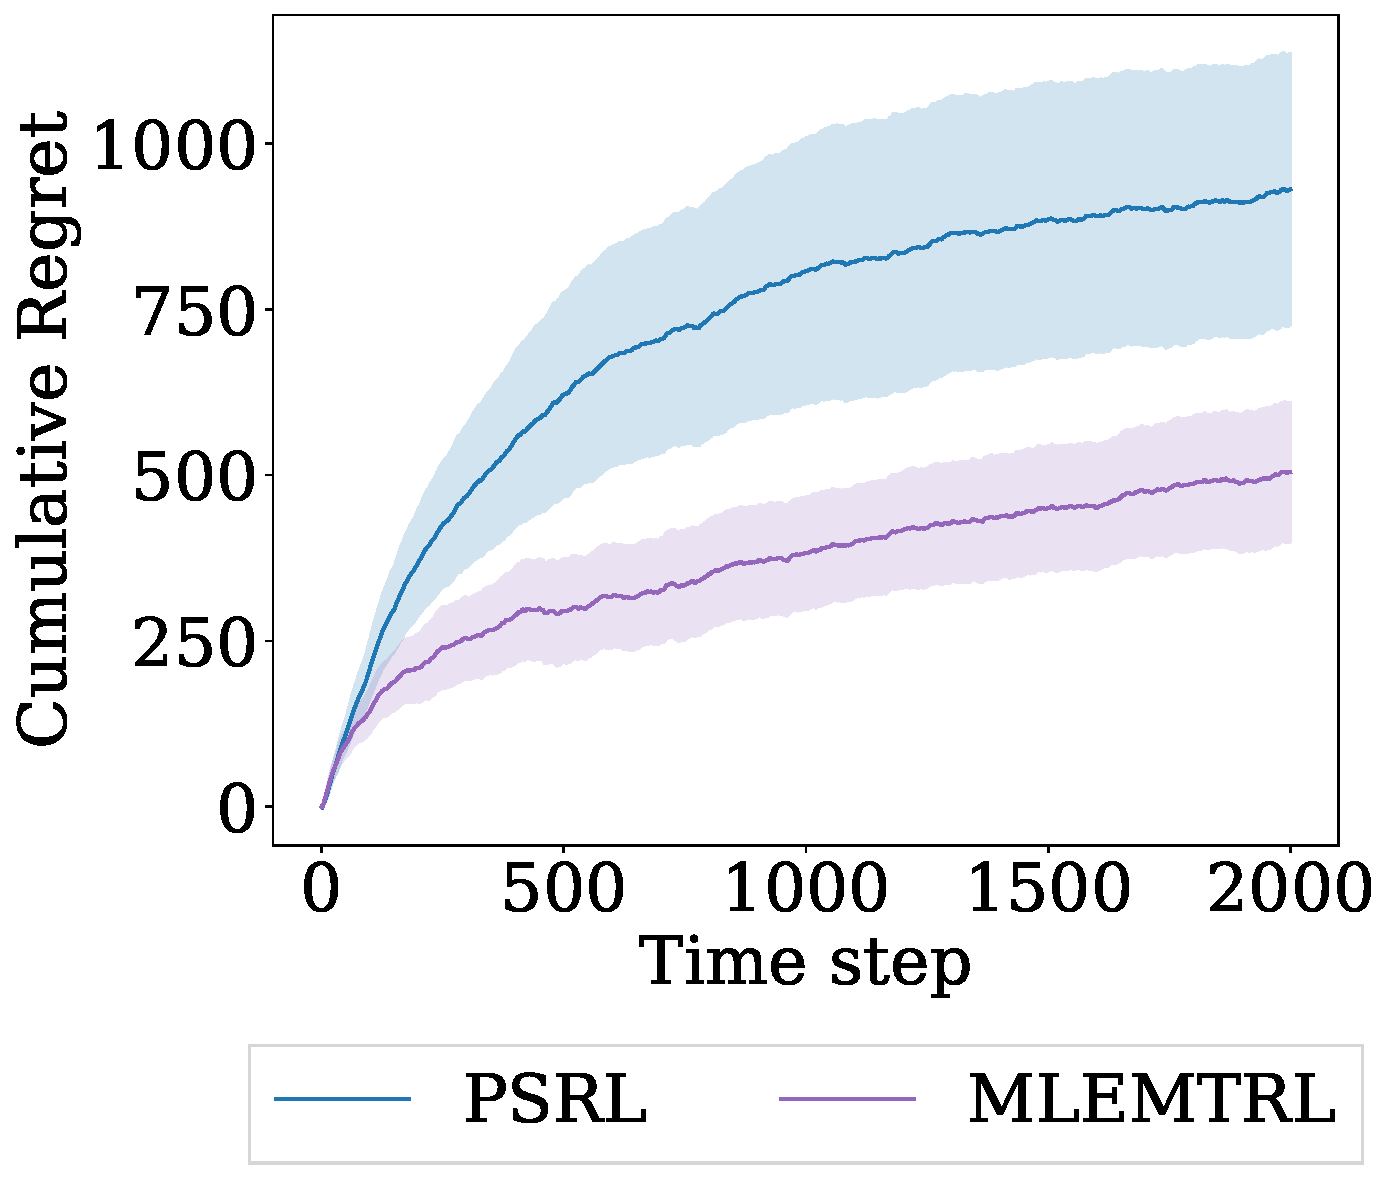
\includegraphics[width=0.4\textwidth]{img/chain_experiment.pdf}
%    \caption{This visualisation is of multiple variants of the Chain environment. Here, the slippage parameter is being varied. The cumulative regret is shown over the first $2000$ time steps and the shaded regions represent the $95\%$ confidence interval of the cumulative regret for the two algorithms. The agents update their policies every $20$ steps. For regret, lower values are better.}\label{fig:chain}\vspace*{-1em}
%\end{figure}
%\fi

\setlength{\textfloatsep}{4pt}%
\begin{figure}[t!]
    \centering
    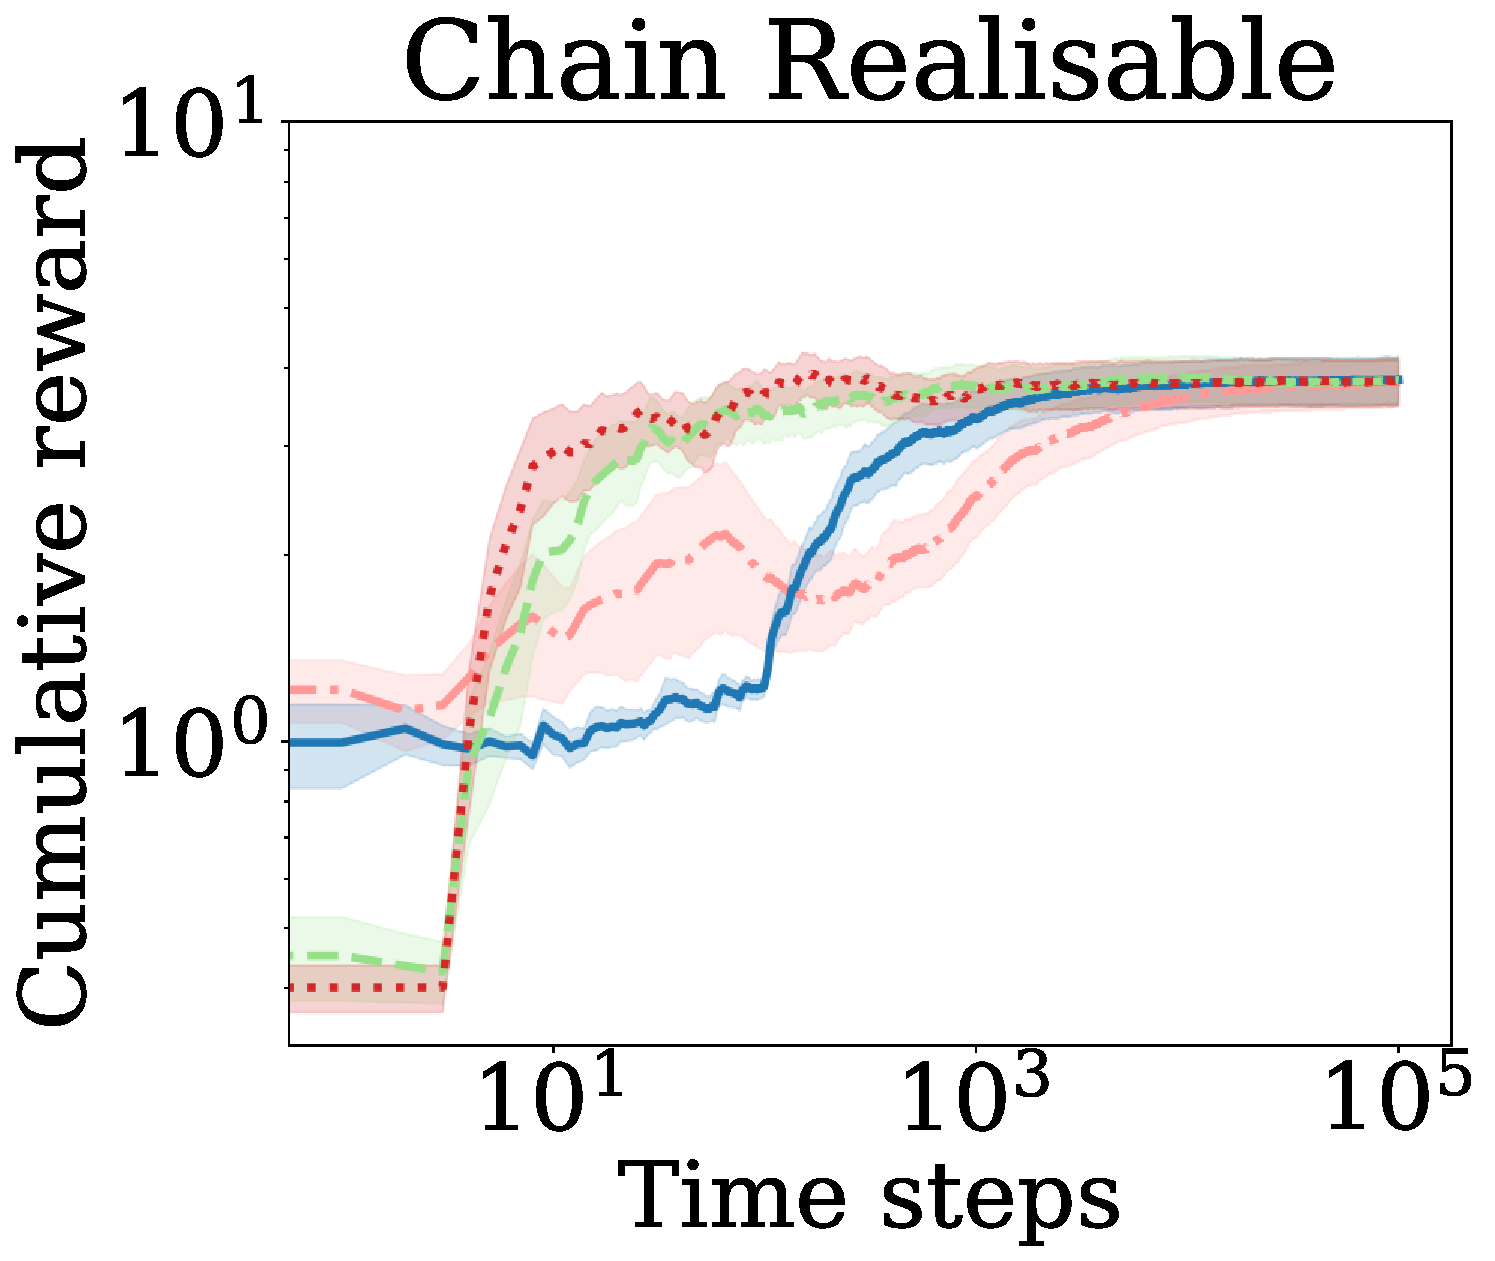
\includegraphics[width=0.3\textwidth]{img/chain_realisable.pdf}         
    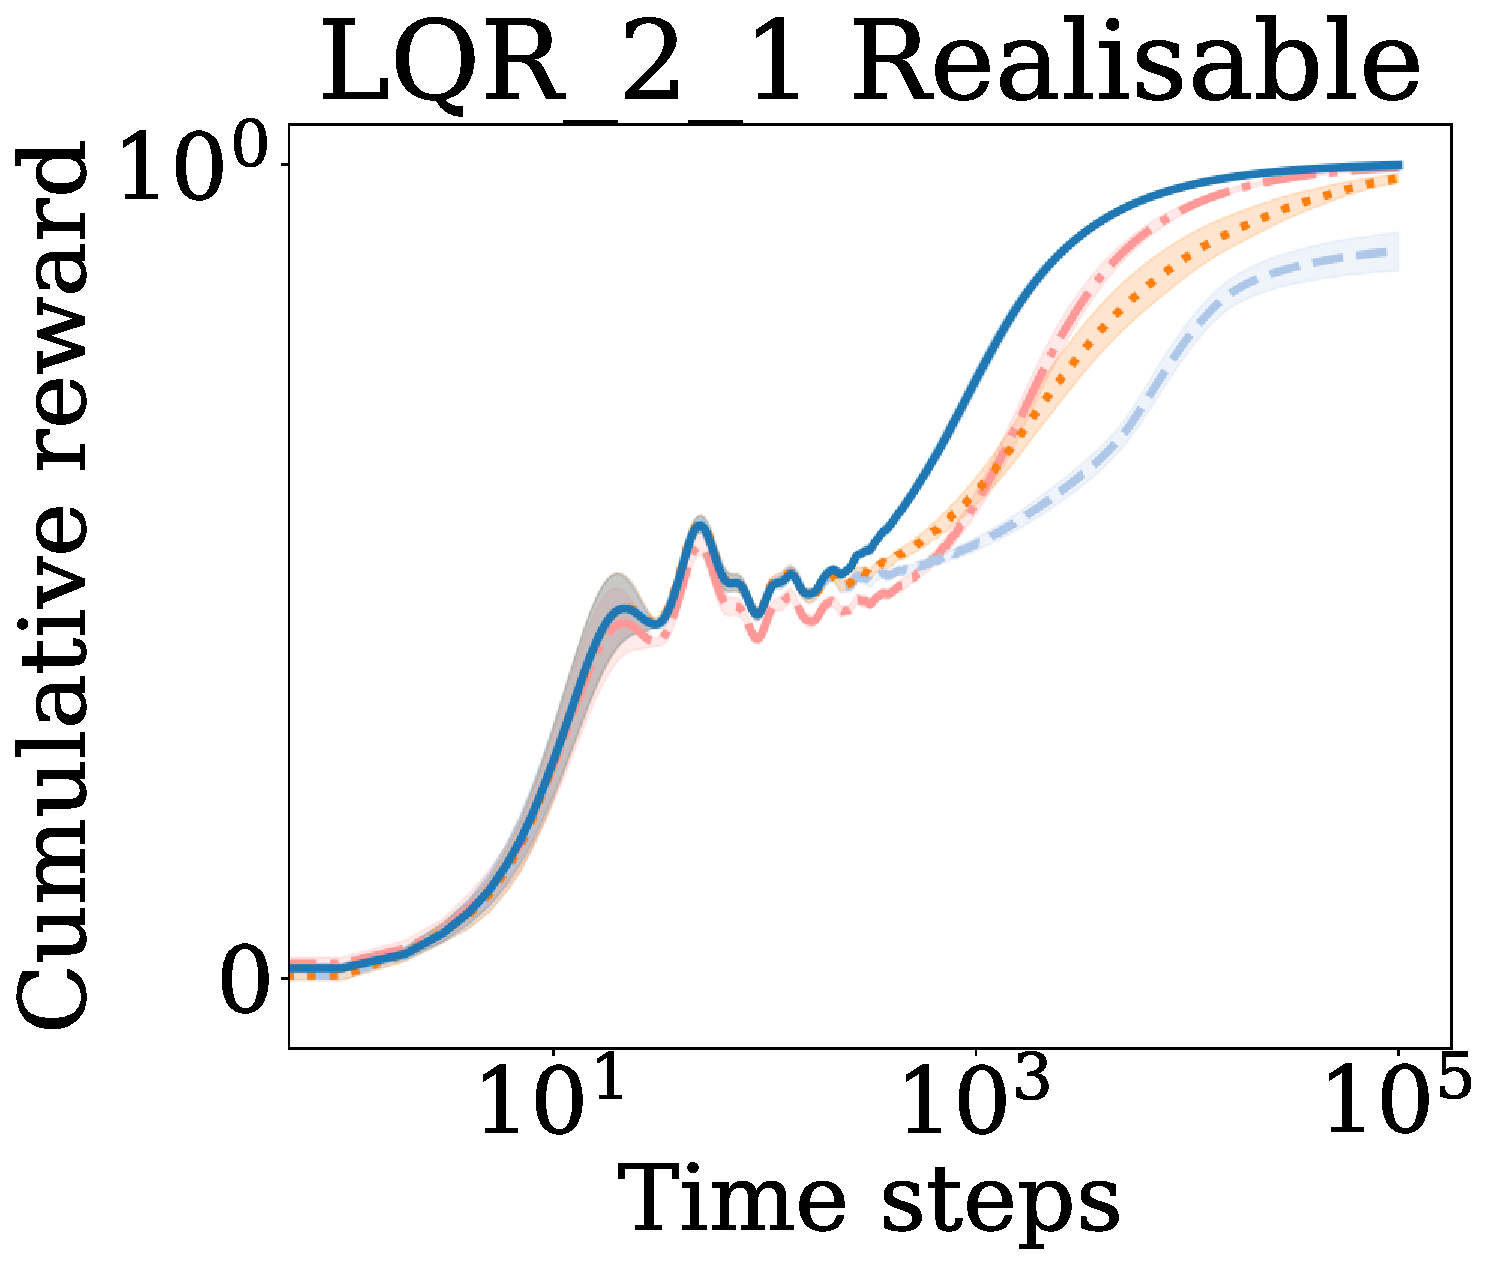
\includegraphics[width=0.3\textwidth]{img/lqr_2_1_realisable.pdf} 
    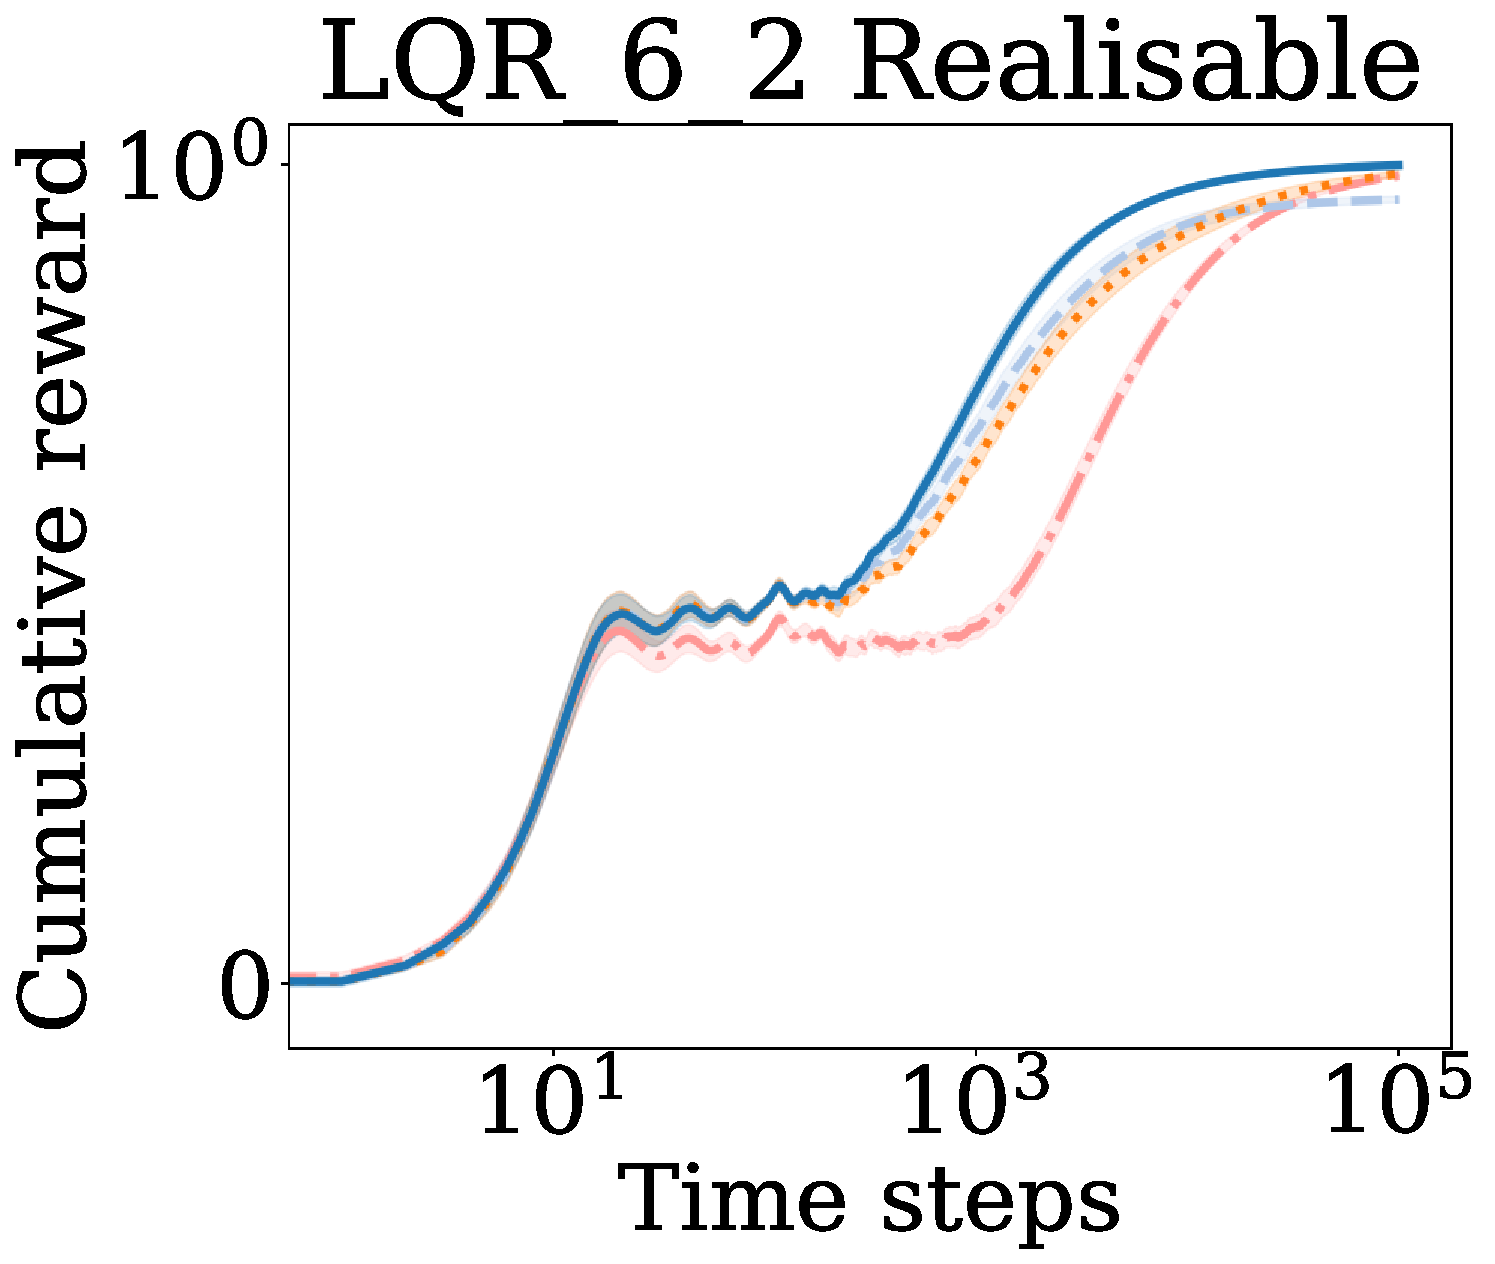
\includegraphics[width=0.3\textwidth]{img/lqr_6_2_realisable.pdf}\\
    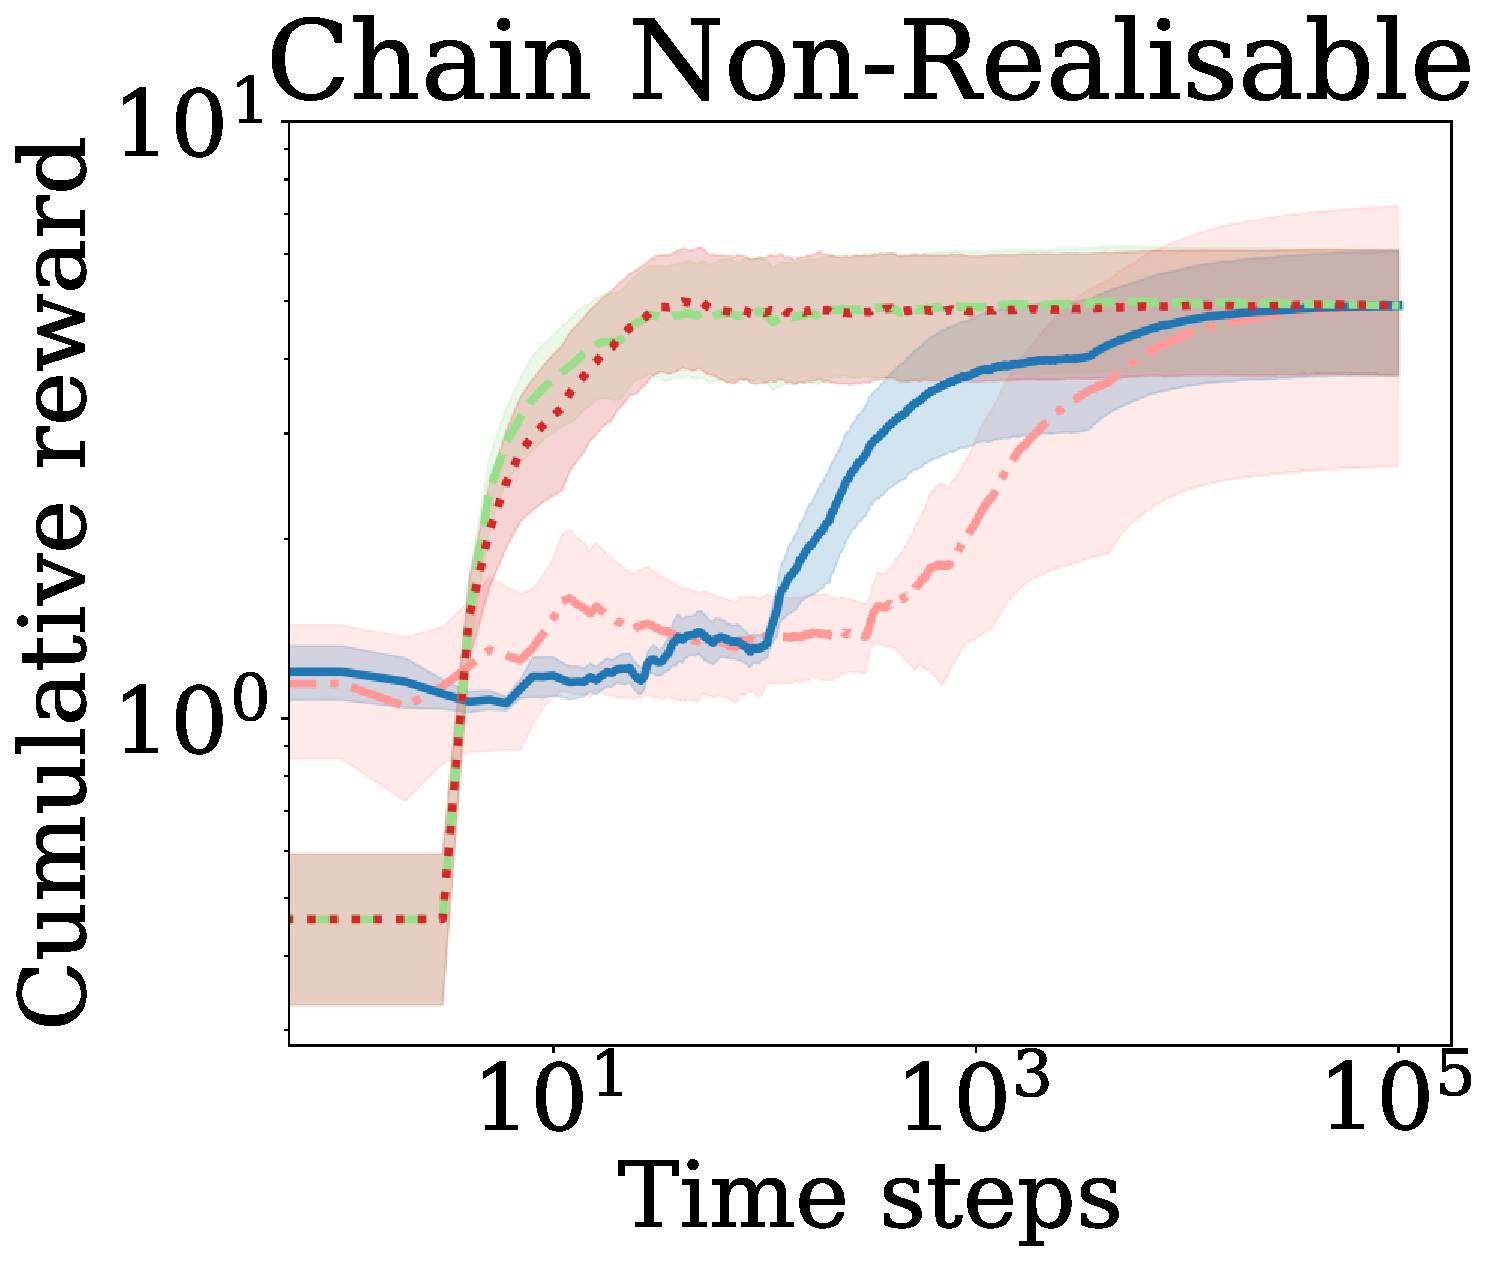
\includegraphics[width=0.3\textwidth]{img/chain_non_realisable.pdf}        
    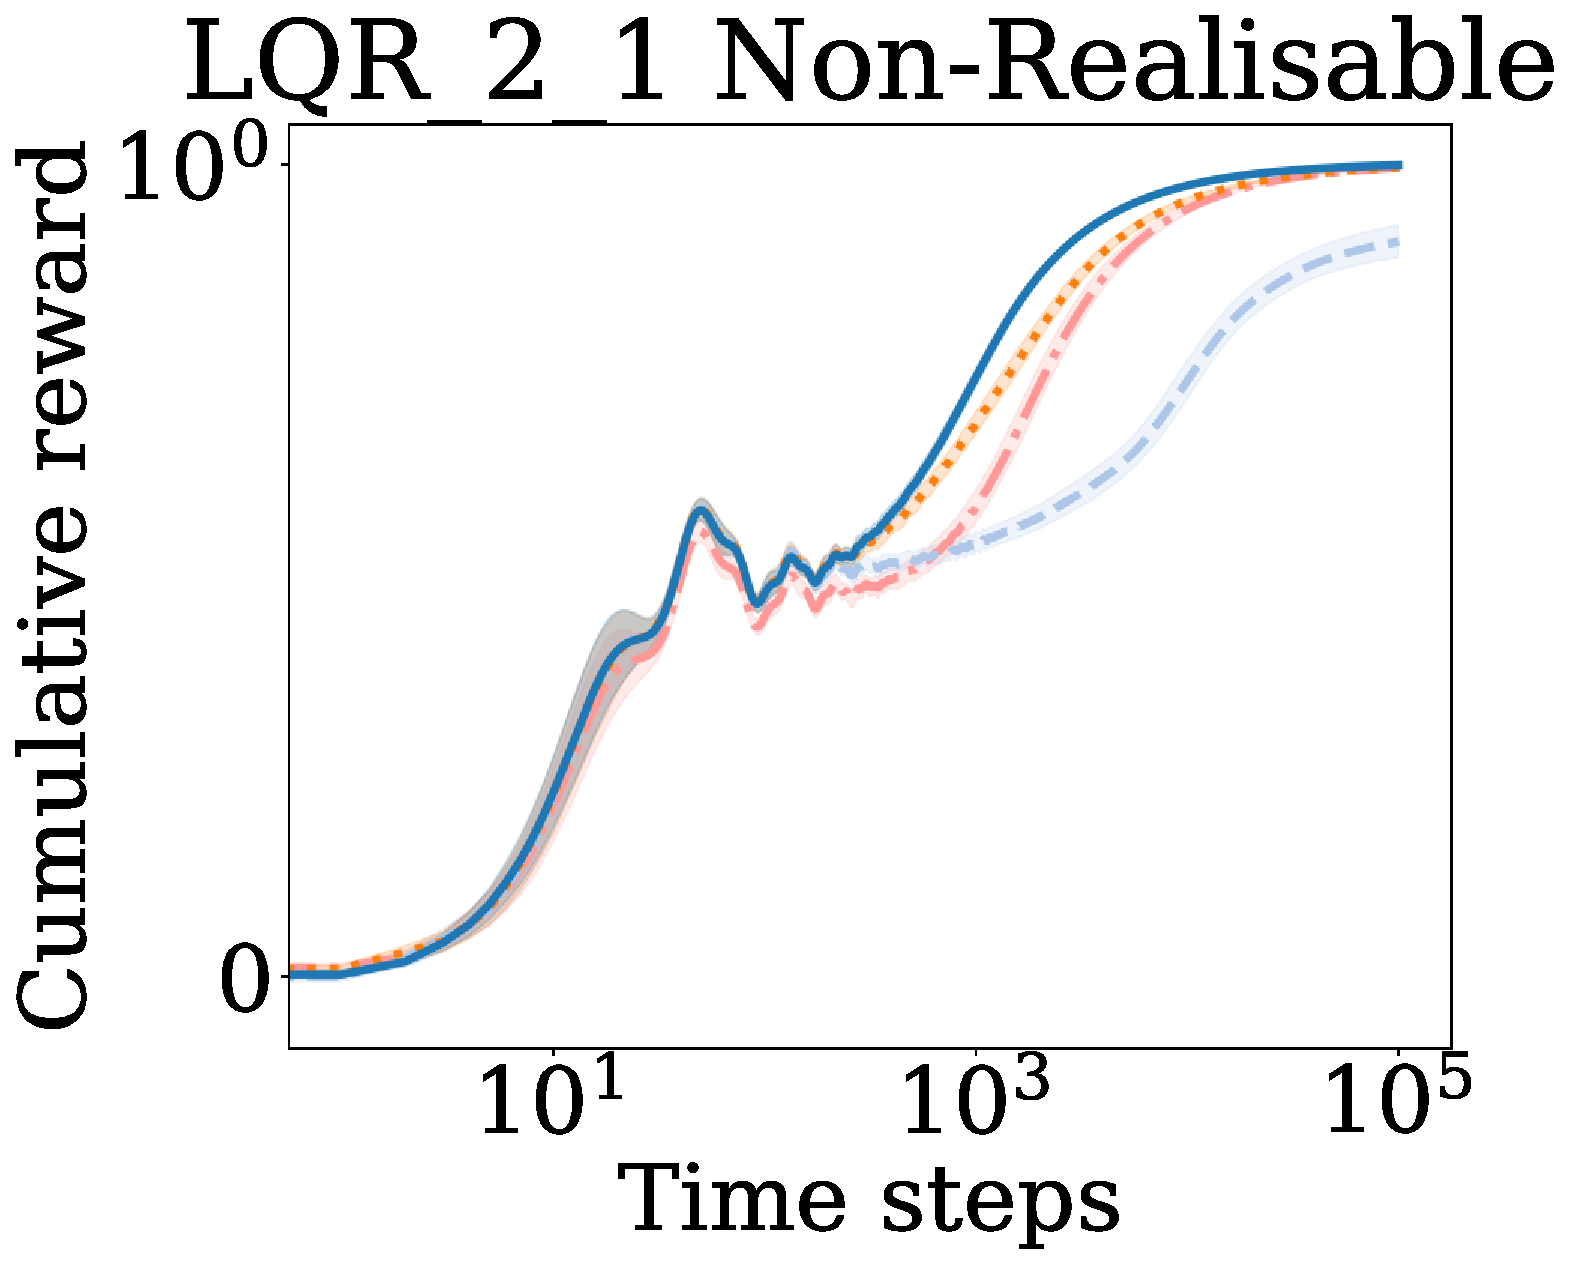
\includegraphics[width=0.3\textwidth]{img/lqr_2_1_non_realisable.pdf} 
    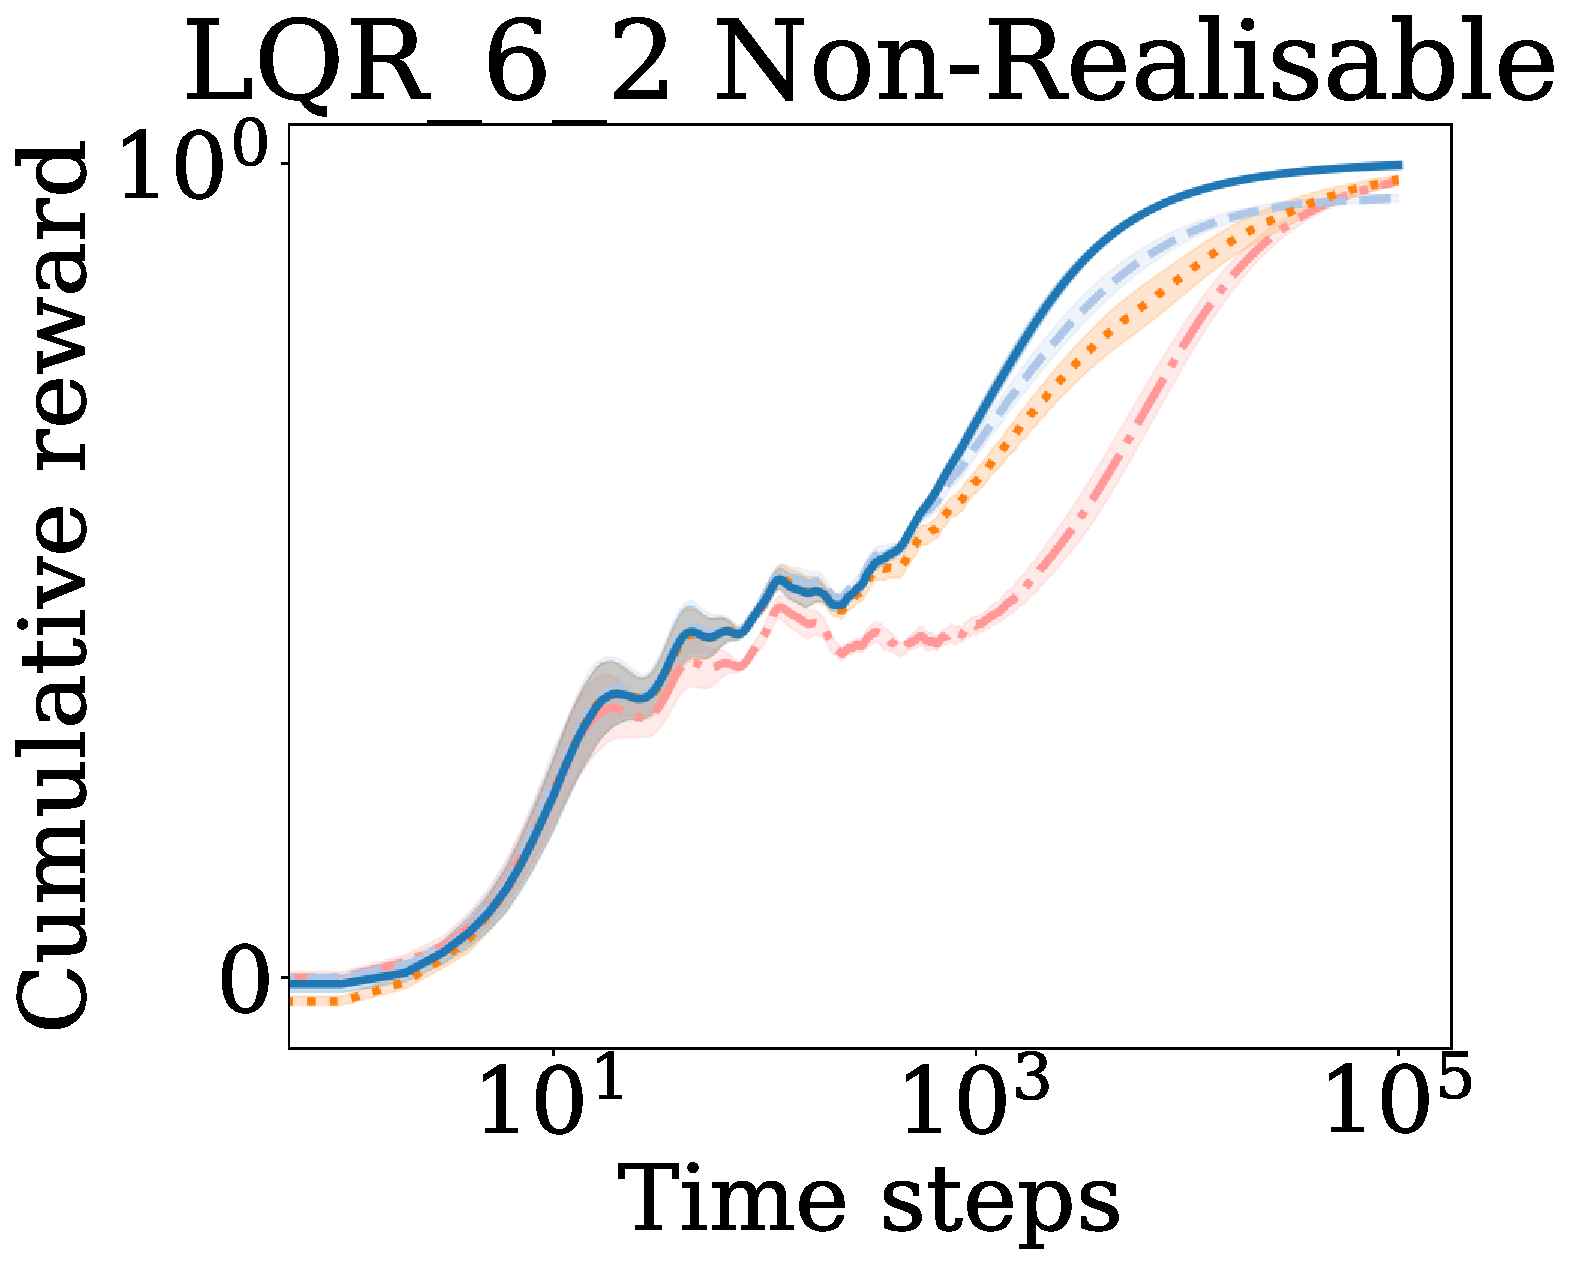
\includegraphics[width=0.3\textwidth]{img/lqr_6_2_non_realisable.pdf}\\
    
\includegraphics[width=0.9\textwidth]{img/lqr_legend.pdf}
    \caption{Depicted is the average cumulative reward at every time step computed over $10$ novel tasks in the realisable/non-realisable setting. The shaded regions represent the standard error of the average cumulative reward at the time step.}\label{fig:full_results}%\vspace*{-1em}
\end{figure}


\noindent\textbf{RL Environments.} We test the algorithms in a tabular MDP, i.e. Chain~\citep{dearden1998bayesian}, CartPole~\citep{barto1983neuronlike}, and two LQR tasks in \emph{Deepmind Control Suite}~\citep{tassa2018deepmind}: \emph{dm\_LQR\_2\_1} and \emph{dm\_LQR\_6\_2}. %Further details on experimental setups are deferred to Appendix~\ref{sec:rl_env}.
Further details on experimental setups are deferred to Appendix C.1.


\noindent\textbf{(1) Impacts of Model Transfer with MLEMTRL.}\label{sec:impacts} We begin by evaluating the proposed algorithm in the Chain environment. The results of the said experiment are available in the leftmost column of Figure~\ref{fig:full_results}. In it, we evaluate the performance of MLEMTRL against PSRL, MT-PPO, MT-PPO-TRL. The experiments are done by varying the slippage parameter $p \in [0.00, 0.50]$ and the results are computed for each different setup of Chain from scratch. In this experiment, we can see the baseline algorithms MT-PPO and MT-PPO-TRL perform very well. This could partially be explained by PSRL and MLEMTRL not only having to learn the transition distribution but also the reward function. The value function transfer in the PPO-based baselines implicitly transfers not only the empirical transition model but also the reward function. We can see that MLEMTRL has improved learning speed compared to PSRL in both realisable and non-realisable settings. 
An additional experiment with a known reward function across tasks is shown in %Figure~\ref{fig:known_reward_results}. 
Figure 7 in Appendix.
%An additional experiment with known reward function across tasks is shown in Figure~\ref{fig:known_reward_results}. 

In the centre and rightmost columns of Figure~\ref{fig:full_results}, we can see the results of running the algorithms in the LQR settings with the baseline algorithms PSRL, MT-SAC and MT-SAC-TRL. The variation over tasks is given by the randomness over the stiffness of the joints in the problem. In these experiments, we can see a clear advantage of MLEMTRL compared to all baselines in terms of learning speed improvements, and in some cases, asymptotic performance.

In Figure~\ref{fig:full_results}, the performance metric is the average cumulative reward at every time step, for $10^5$ time steps and the shaded region represents the standard deviation, where the statistics are computed over $10$ independent tasks. %\\

%The average cumulative reward  and the shaded regions represent the $95\%$ confidence of the cumulative regret at the time step. The confidence interval is taken over the various variations of the Chain environment. The image clearly shows MLEMTRL has a jumpstart improvement coming as a result of the transfer learning scheme but also an indication of a learning speed improvement. 

\noindent\textbf{(2) Impact of Realisability Gap on Regret.} Now, we further illustrate the observed relation between model dissimilarity and degradation in performance. Figure~\ref{fig:norms} depicts the regret against the KL-divergence of the target model to the best proxy model in the convex set. We observe that model dissimilarity influences the performance gap in MLEMTRL. This is also justified in Section~\ref{sec:bounds} where the bounds have an explicit dependency on the model difference. In this figure, only the non-zero regret experiments are shown. This is to have an idea of which models result in poor performance. As its shown, it is those models that are very dissimilar. Additional results in %Figure~\ref{fig:time} further illustrate the dependency on model similarity.%\\
% Figure 5 in Appendix further illustrate the dependency on model similarity.


\begin{figure}[h]
    \centering
    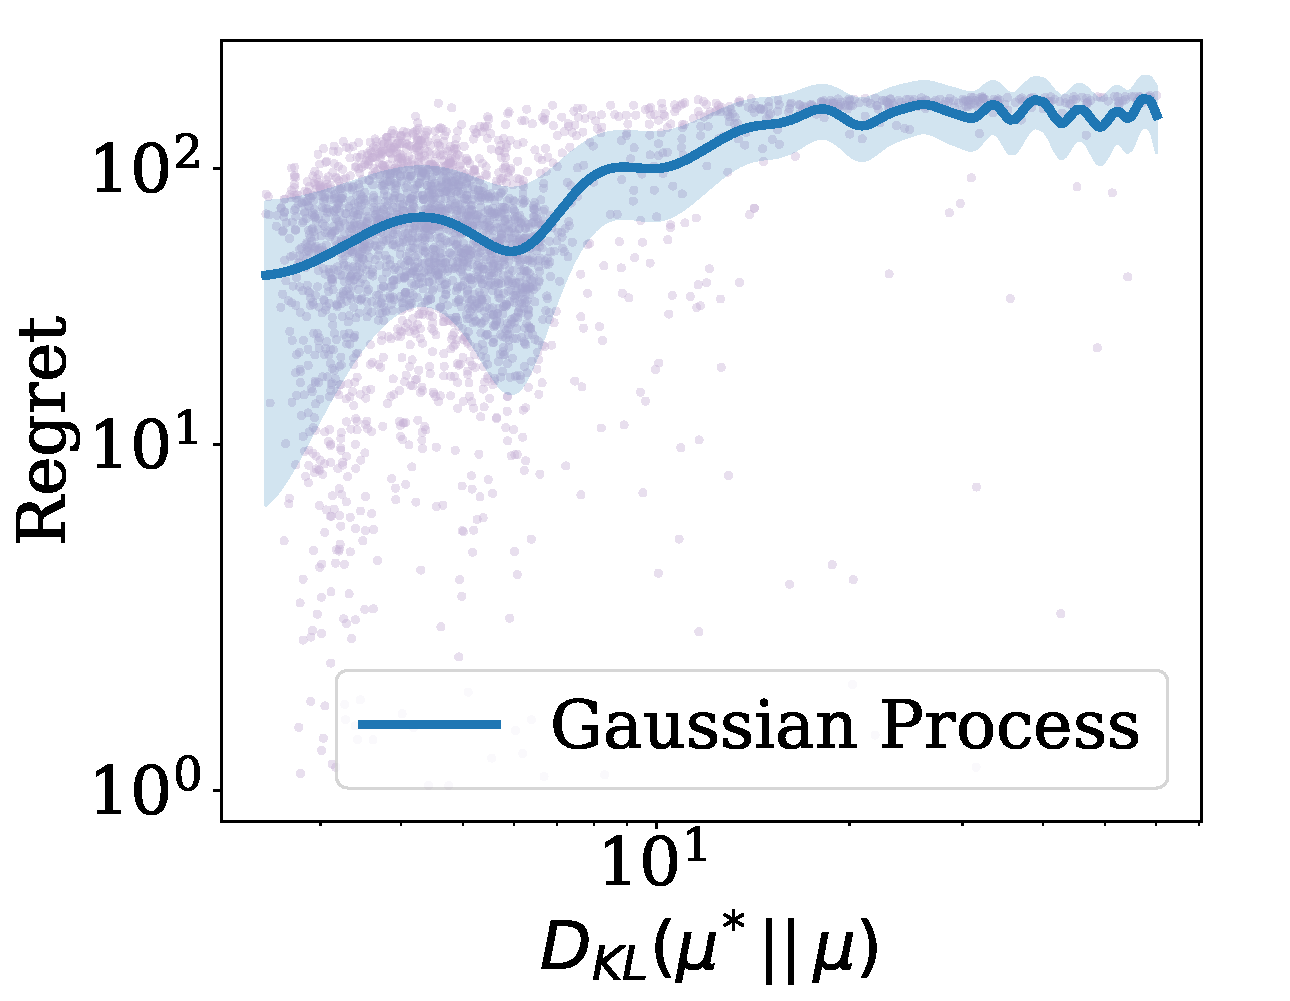
\includegraphics[width=.5\textwidth]{img/alpha_norms}
    \caption{A log-log plot of regret vs. KL-divergence between the true MDP and the best proxy model in CartPole. The thick blue line is a Gaussian Process regression model fitted on observed data (in purple).}
    \label{fig:norms}
\end{figure}

\begin{figure}[h]
    
    \centering
    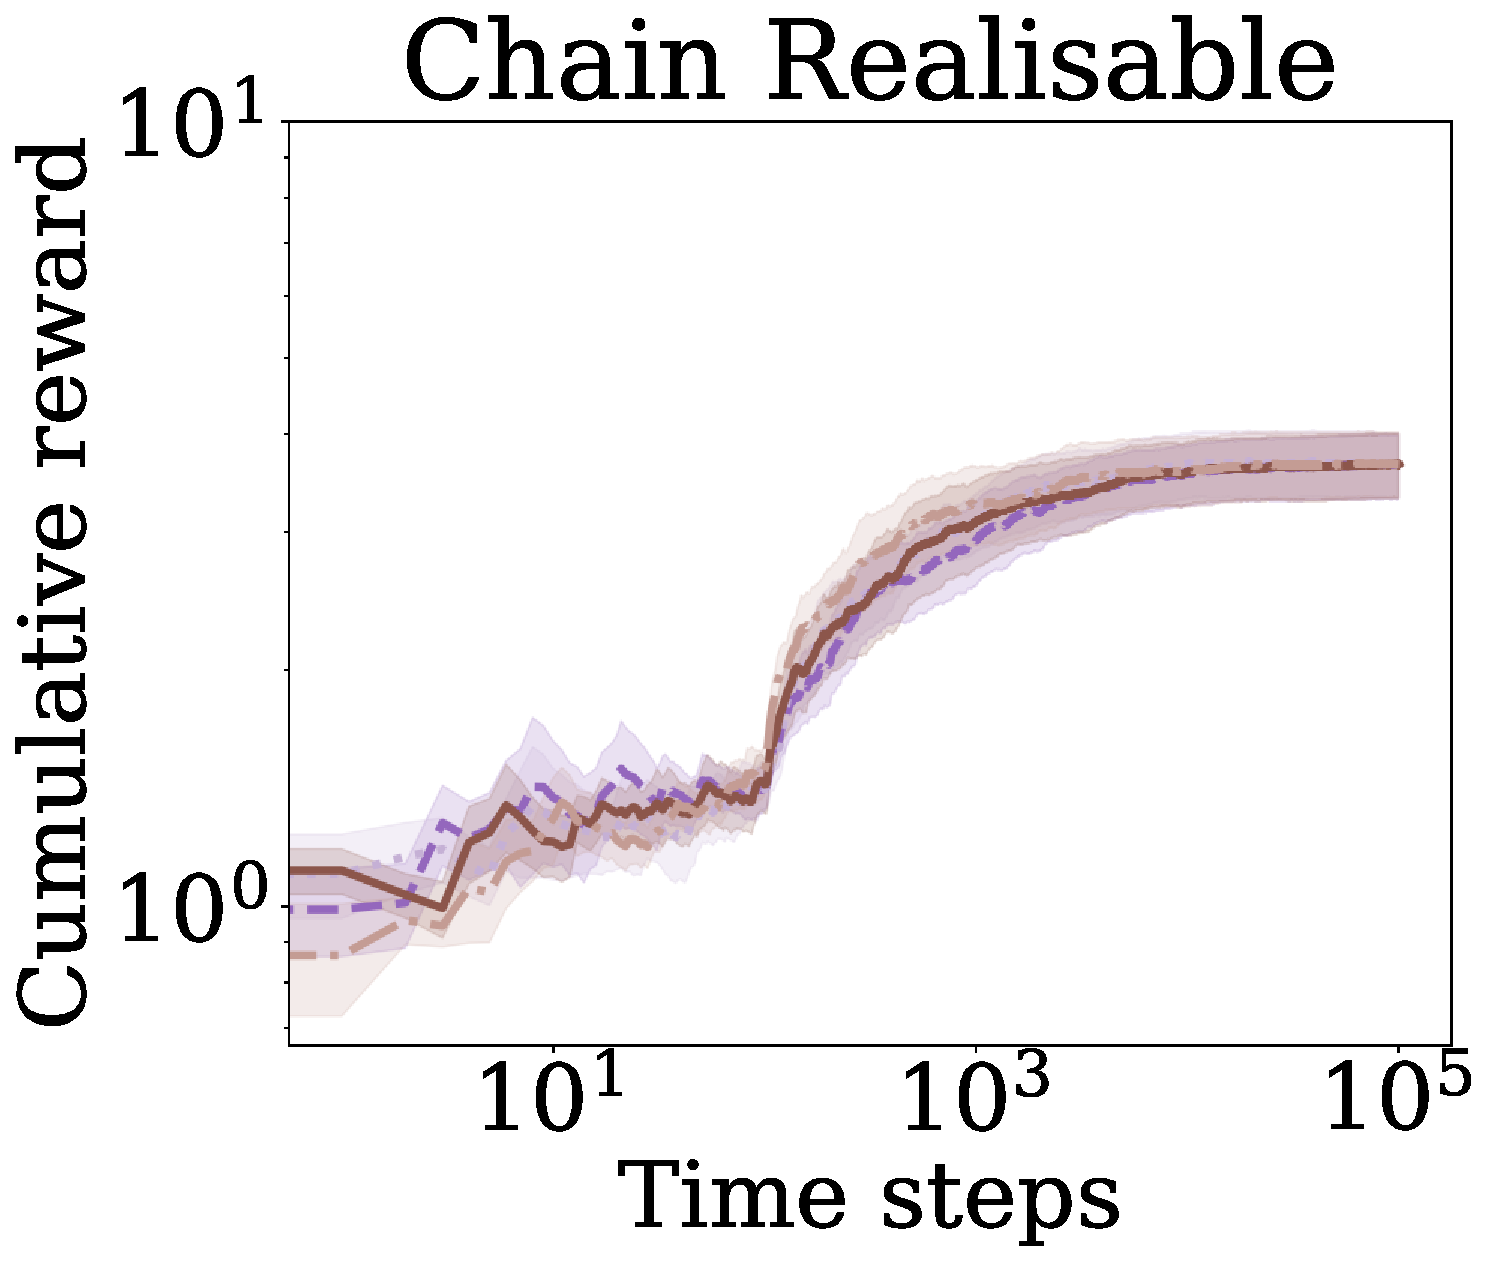
\includegraphics[width=0.48\textwidth]{img/chain_meta_realisable.pdf} 
    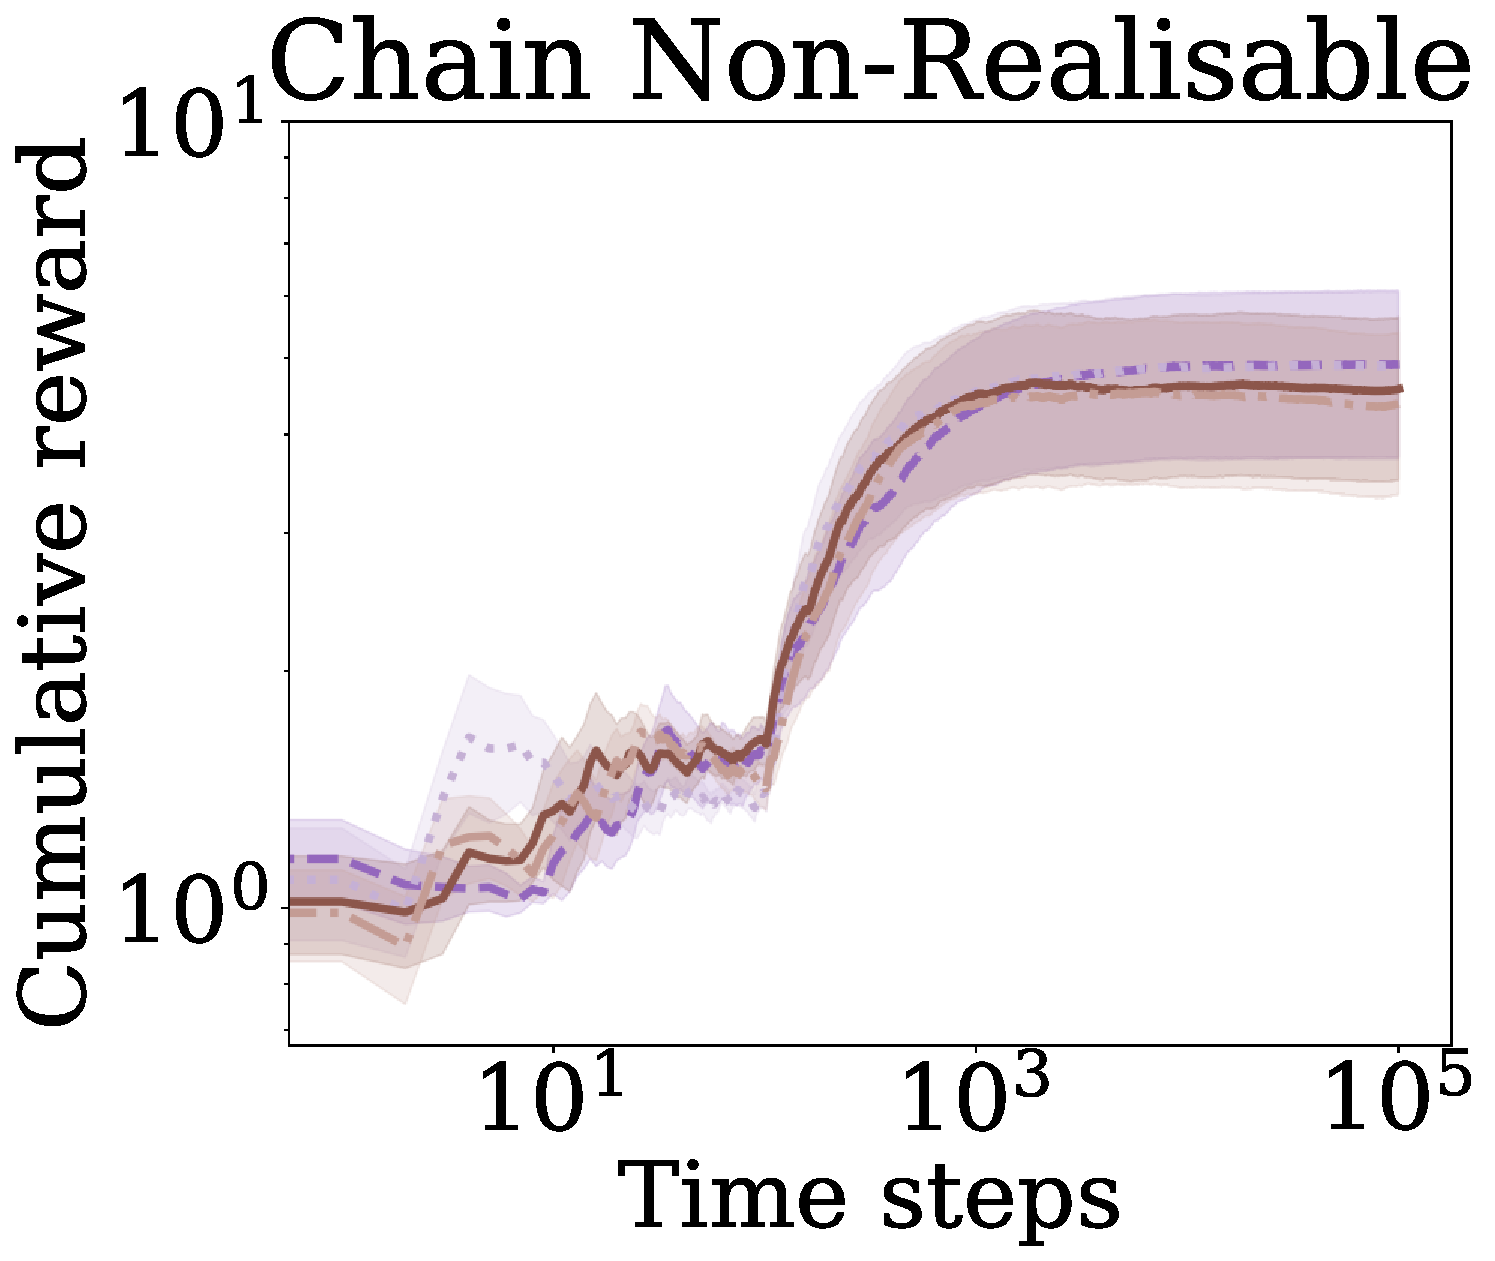
\includegraphics[width=0.48\textwidth]{img/chain_meta_non_realisable.pdf}\\
    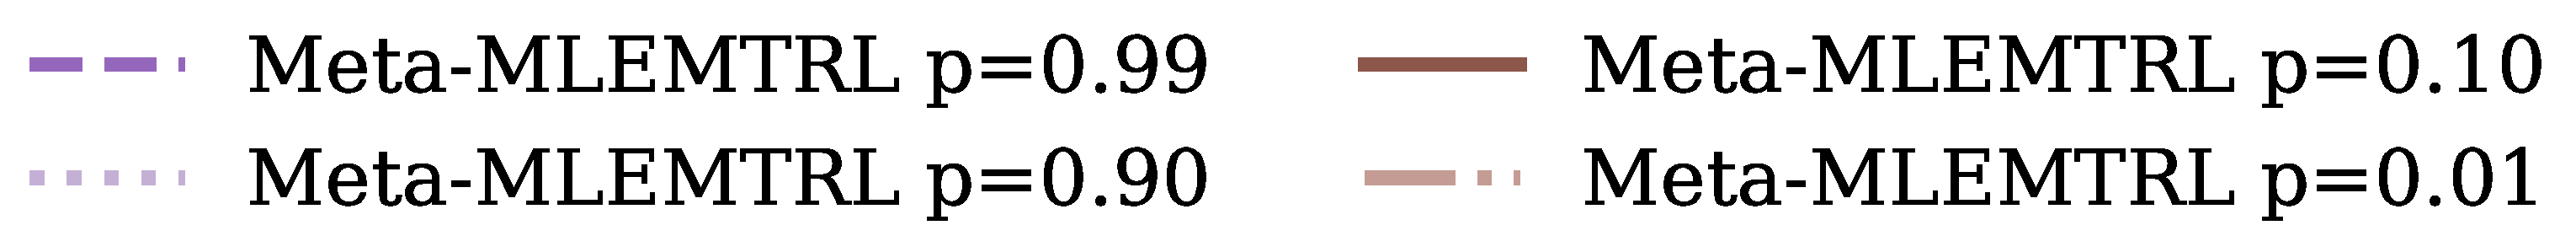
\includegraphics[width=0.9\textwidth]{img/lqr_legend3.pdf}
    \caption{Figure depicting an ablation study of the prior parameter $p$ in the Meta-MLEMTRL algorithm. The y-axis is the average cumulative reward at each time step computed over $10$ novel tasks and the shaded region represents the standard error. When $p=1$, the algorithm reduces to MLEMTRL and when $p=0$ the algorithm reduces to standard maximum likelihood model estimation.}
    \label{fig:meta_results}
\end{figure}


% \begin{figure*}[t!]
% \centering
%     \begin{minipage}{0.34\textwidth}
%     \centering
%     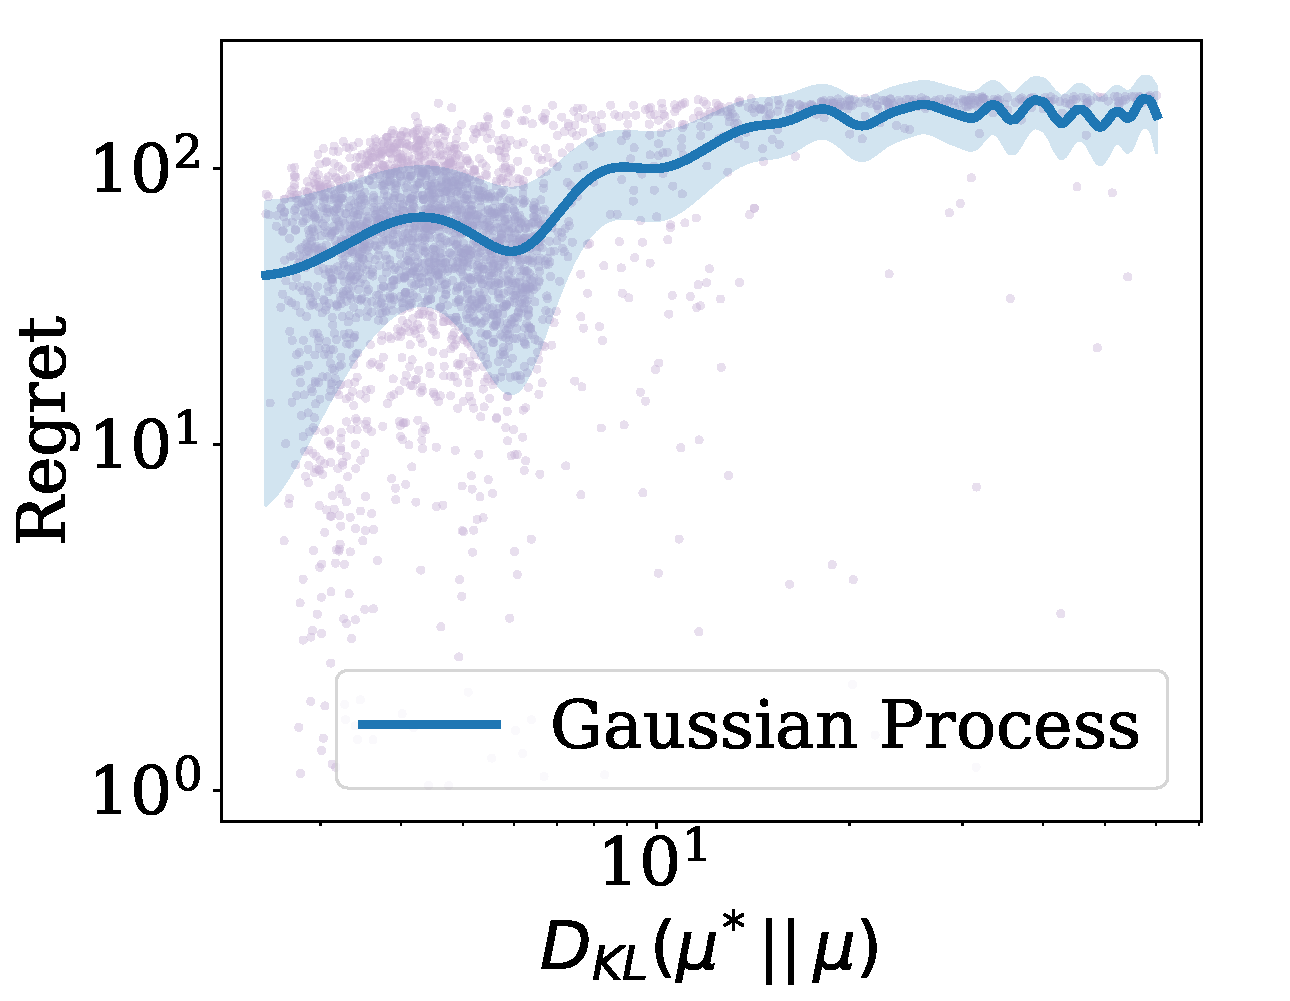
\includegraphics[width=\textwidth]{img/alpha_norms}\\~\\~\\
%     \caption{A log-log plot of regret vs. KL-divergence between the true MDP and the best proxy model in CartPole. The thick blue line is a Gaussian Process regression model fitted on observed data (in purple).}\label{fig:norms}%Only the non-zero regret results are displayed to indicate how sub-optimal performance relates to model dissimilarity. 
%     \end{minipage}\hfill
%     \begin{minipage}{0.65\textwidth}
%     \centering
%     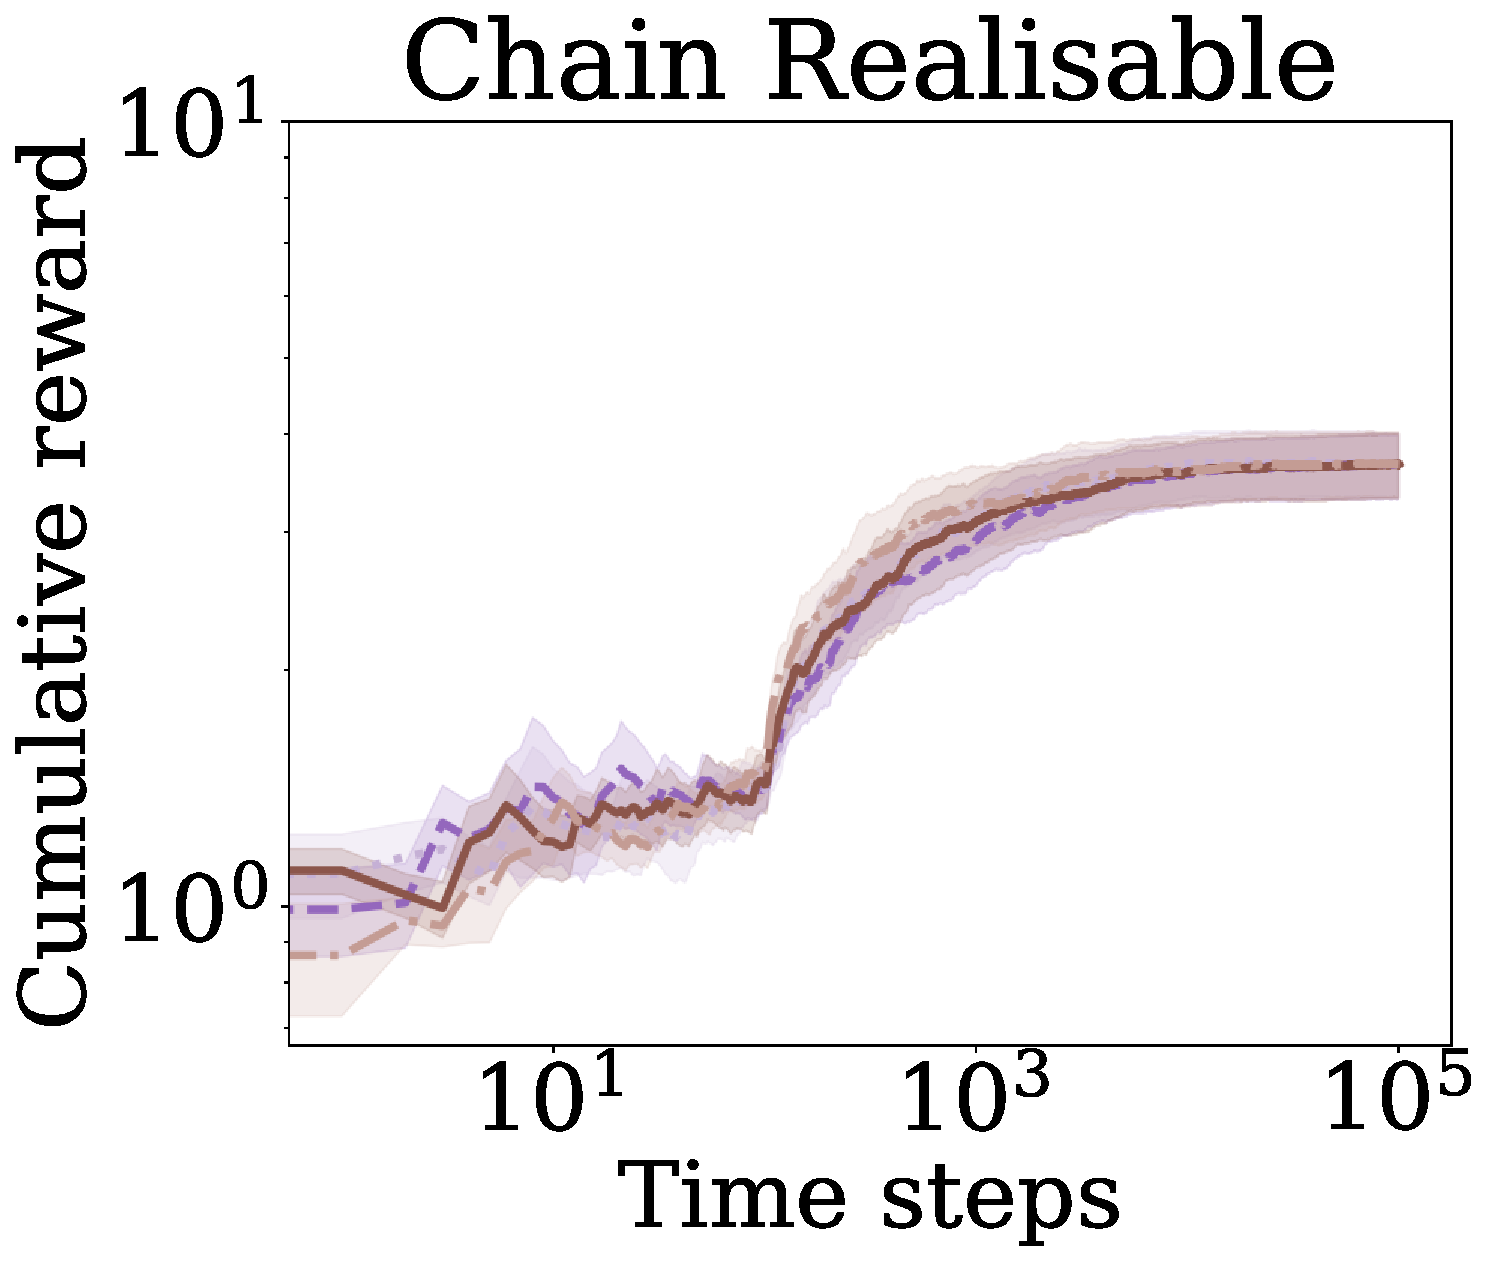
\includegraphics[width=0.48\textwidth]{img/chain_meta_realisable.pdf} 
%     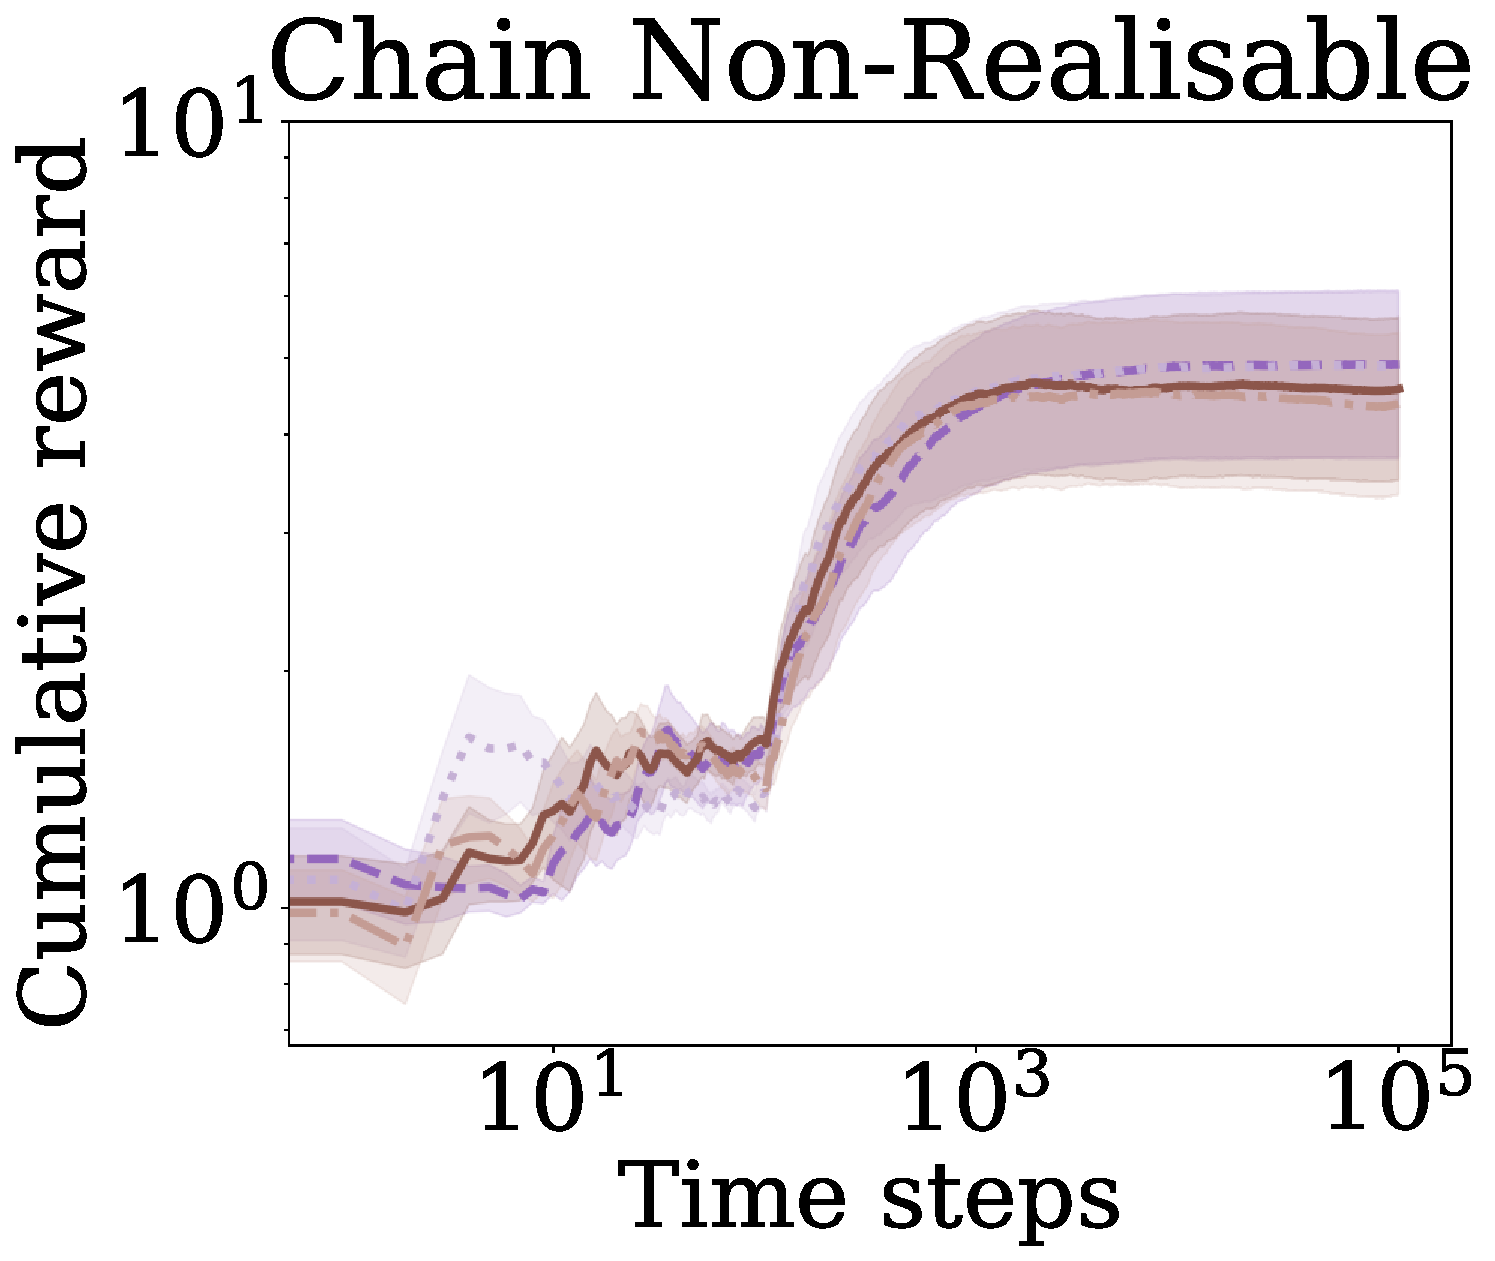
\includegraphics[width=0.48\textwidth]{img/chain_meta_non_realisable.pdf}\\
%     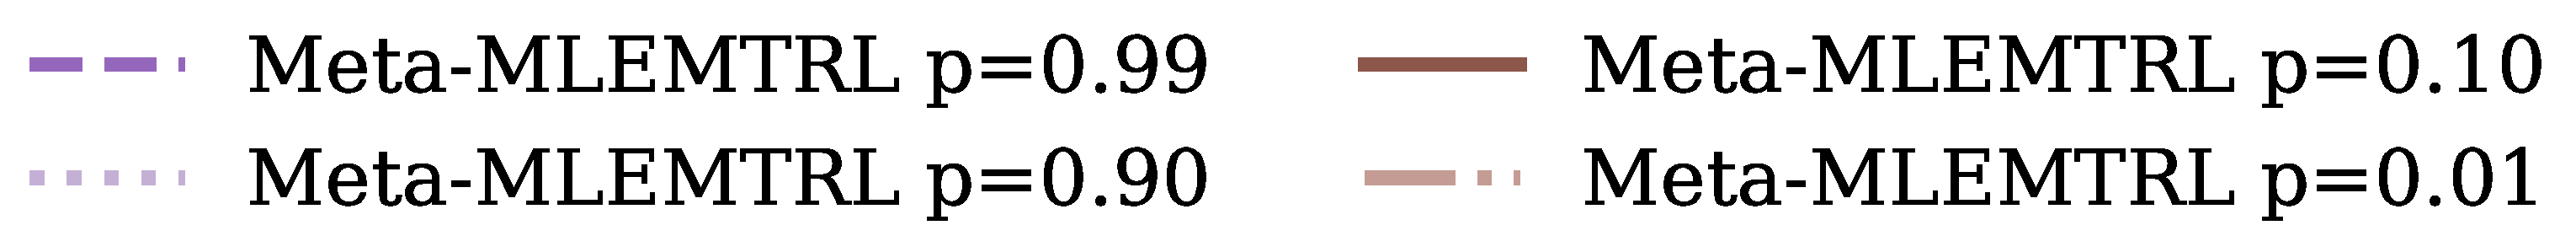
\includegraphics[width=0.9\textwidth]{img/lqr_legend3.pdf}
%     \caption{Figure depicting an ablation study of the prior parameter $p$ in the Meta-MLEMTRL algorithm. The y-axis is the average cumulative reward at each time step computed over $10$ novel tasks and the shaded region represents the standard error. When $p=1$, the algorithm reduces to MLEMTRL and when $p=0$ the algorithm reduces to standard maximum likelihood model estimation.}\label{fig:meta_results}
%     \end{minipage}
% \end{figure*}

\noindent\textbf{(3) Performance of Meta-MLEMTRL under Non-realisability.} In order to validate the performance of the proposed meta algorithm Meta-MLEMTRL, we perform an ablation study over the prior hyperparameter $p$. In Figure~\ref{fig:meta_results}, we illustrate the results of running the Meta-MLEMTRL algorithm in the Chain environment for both the realisable and non-realisable settings. The choice of $p$ determines how much the algorithm should be biased towards the model estimated using MLEMTRL and in the case when $p=1$, Meta-MLEMTRL reduces to MLEMTRL. Similarly, if $p=0$ then the algorithm will forego the MLEMTRL-estimate for the empirical estimate. Figure~\ref{fig:meta_results} shows that the performance of Meta-MLEMTRL is stable in long-run for different values of $p$. %More experiments would be needed in order to make any strong empirical claims, 
However, we identify that higher $p$ values yield positive improvements in the cumulative reward over $10^5$ steps, especially in the non-realisable setting. This indicates that the MLEMTRL-estimated model acts a good representation, while combined with the asymptotically converging empirical estimate obtained by Meta-MLEMTRL.%\\

\noindent\textbf{Summary of Results.} In the experiments, we sought to identify whether the proposed algorithm shows superiority in terms of the transfer learning goals given by~\citep{langley2006transfer}. In the LQR-based environments, we can see a clear superiority of MLEMTRL in terms of learning speed compared to all baselines and in some cases, an asymptotic improvement. In the Chain environment, the proposed algorithm, MLEMTRL, outperforms PSRL in terms of learning speed. Also, we perform an ablation study of Meta-MLEMTRL under realisable and non-realisable settings, demonstrating provable improvements in the asymptotic and non-realisable regimes.

%In our first experiment, we see a clear superiority in terms of learning speed and jumpstart improvement. These results are consistent for the second experiment as well, given that the true MDP is similar enough to the source tasks. In the second and third experiment we verify the claim that a loss in performance (in terms of regret) has a strong dependence on the dissimilarity of the estimated MDP and the true MDP.

%Additional ablative experiments showing how the performance loss increases with model dissimilarity is available in Figure~\ref{fig:norms}, how MLEMTRL can be augmented with an hierarchical procedure to take the empirical model into account in addition to the source models in Figure~\ref{fig:meta_results} and in Figure~\ref{fig:sac_results}, showing how the use of multi-task and transfer reinforcement learning may improve the performance over a standard RL approach.

%Additional ablation studies showing how MLEMTRL can be augmented with a hierarchical procedure to take the empirical model into account in addition to the source models are depicted in Figures~\ref{fig:meta_results} and~\ref{fig:sac_results}. They show how the use of multi-task and transfer RL can improve performance over a standard RL approach. 

%Additional ablative experiments showing how MLEMTRL can be augmented with an hierarchical procedure to take the empirical model into account in addition to the source models in Figure 4 and in Figure 5, showing how the use of multi-task and transfer reinforcement learning may improve the performance over a standard RL approach.


\section{Discussions and Future Work}\label{sec:discussion}
In this work, we aim to answer two central questions.
%1. \emph{How can we accurately construct a model using a set of source models for an RL agent deployed in the wild?}
% 2. \emph{Does the constructed model allows us to perform efficient planning and yield improvements over learning from scratch?} 
\begin{enumerate}
   \item \emph{How can we accurately construct a model using a set of source models for an RL agent deployed in the wild?}
   \item \emph{Does the constructed model allow us to perform efficient planning and yield improvements over learning from scratch?}
\end{enumerate}

Our answer to the first question is by adopting the \emph{Model Transfer Reinforcement Learning} framework and weighting existing knowledge together with data from the novel task. We accomplished this by following a maximum likelihood-based approach. This has led to a novel algorithm, MLEMTRL, consisting of a model identification stage and a model-based planning stage. 
The second question is answered by the empirical results in Section~\ref{sec:experiments} and the theoretical results in Section~\ref{sec:bounds}. Further, the model allows generalising to novel tasks, given that the tasks are similar enough to the existing task(s). 

We motivate the use of our framework in settings where an agent is to be deployed in a new domain that is similar to existing, known, domains. We verify the quick, near-optimal performance of the algorithm in the case where the new domain is similar and we prove worst-case performance bounds of the algorithm in both the realisable and non-realisable settings.
As a future work, it would be interesting to study the MTRL framework under Bayesian setting~\citep{tamar2022regularization} and to deploy it with a risk-sensitive value function~\citep{eriksson2022sentinel,saac}.

\section*{ACKNOWLEDGMENTS}
This work was partially supported by the Wallenberg AI, Autonomous Systems and Software Program (WASP) funded by the Knut and Alice Wallenberg Foundation. D. Basu acknowledges the Inria-Kyoto University Associate Team “RELIANT” and the ANR JCJC grant for the REPUBLIC project (ANR22-CE23-0003-01).


% \balance
% balance should be at the end of last page to balance citations
%We motivate the use of our framework in settings where an agent is to be deployed in a new domain that is similar to existing, known, domains. We verify the relation of the \emph{regret} w.r.t the model dissimilarity in terms of KL-divergence and the quick, near-optimal performance of the algorithm in the case where the new domain is similar. In addition to this, we prove worst-case performance bounds of the algorithm in both the realisable and non-realisable settings. 

%%% balances text on the left column of the final page!

%%%
%\textit{Future work.} An interesting future work is to derive tighter bounds for the \emph{realisable} case in Section~\ref{subsec:realisable}. Note $\delta=0$ in the realisable setting but the large constant $\epsilon$ remains. A concentration bound in the number of samples from the true MDP could be constructed using the proof techniques in~\citet{anastasiou2019normal} and~\citet{ouhamma2022bilinear}. We would also like to investigate larger and more difficult problems. One challenge is devising tractable models in such cases, and to be able to do optimal model-based planning for large scale problems. We would start by considering large problems that can be written as LQR problems, such as~\citep{tunyasuvunakool2020dm_control} and Mujoco~\citep{todorov2012mujoco}.

 

% \begin{acks}
%     This work was partially supported by the Wallenberg AI, Autonomous Systems and Software Program (WASP) funded by the Knut and Alice Wallenberg Foundation and the computations were performed on resources at Chalmers Centre for Computational Science and Engineering (C3SE) provided by the Swedish National Infrastructure for Computing (SNIC).
% \end{acks}




